\documentclass[11pt,a4paper]{article}

% ============================================================
% PACKAGES
% ============================================================
\usepackage[a4paper,margin=1in]{geometry}
\usepackage{fancyhdr}
\usepackage{titlesec}
\usepackage{graphicx}
\usepackage[hidelinks,colorlinks=true,linkcolor=black,citecolor=black,urlcolor=blue]{hyperref}
\usepackage{xcolor}
\usepackage{listings}
\usepackage{tikz}
\usepackage{pgfplots}
\pgfplotsset{compat=1.17}
\usepackage{longtable}
\usepackage{booktabs}
\usepackage{enumitem}
\usepackage{array}
\usepackage{float}
\usepackage{multirow}
\usepackage{caption}
\usepackage{subcaption}
\usepackage{amsmath}
\usepackage{setspace}
\usepackage{tocloft}
\usepackage{lastpage}
\usepackage{pgf-pie}
\usepackage{tabularx}

\usetikzlibrary{shapes,arrows.meta,positioning,fit,backgrounds,calc,decorations.pathreplacing,shadows,trees}

% ============================================================
% COLOR PALETTE
% ============================================================
\definecolor{lumaprimary}{HTML}{2F6690}
\definecolor{lumasecondary}{HTML}{16425B}
\definecolor{lumaaccent}{HTML}{FFA630}
\definecolor{lumalight}{HTML}{E8F1F5}
\definecolor{lumagray}{HTML}{5B5B5B}
\definecolor{lumaok}{HTML}{2E8B57}
\definecolor{lumaerr}{HTML}{C0392B}
\definecolor{codebg}{HTML}{F5F5F5}

% ============================================================
% HEADER / FOOTER
% ============================================================
\pagestyle{fancy}
\fancyhf{}
\renewcommand{\headrulewidth}{0.6pt}
\renewcommand{\footrulewidth}{0.4pt}
\fancyhead[L]{\small\textit{Luma -- Smart Home Monitoring \& Control System}}
\fancyhead[R]{\small\thepage}
\fancyfoot[C]{\small SCS 3311 -- Mobile Application Design and Development}

\fancypagestyle{plain}{%
  \fancyhf{}
  \fancyhead[L]{\small\textit{Luma -- Smart Home Monitoring \& Control System}}
  \fancyhead[R]{\small\thepage}
  \fancyfoot[C]{\small SCS 3311 -- Mobile Application Design and Development}
  \renewcommand{\headrulewidth}{0.6pt}
}

% ============================================================
% SECTION TITLE STYLING
% ============================================================
\titleformat{\section}
  {\normalfont\Large\bfseries\color{lumasecondary}}
  {\thesection}{1em}{}[{\color{lumaprimary}\titlerule[1pt]}]
\titleformat{\subsection}
  {\normalfont\large\bfseries\color{lumaprimary}}
  {\thesubsection}{1em}{}
\titleformat{\subsubsection}
  {\normalfont\normalsize\bfseries\color{lumasecondary}}
  {\thesubsubsection}{1em}{}

% ============================================================
% LISTINGS STYLE
% ============================================================
\lstdefinestyle{codestyle}{
    backgroundcolor=\color{codebg},
    commentstyle=\color{lumagray}\itshape,
    keywordstyle=\color{lumasecondary}\bfseries,
    numberstyle=\tiny\color{lumagray},
    stringstyle=\color{lumaok},
    basicstyle=\ttfamily\footnotesize,
    breakatwhitespace=false,
    breaklines=true,
    captionpos=b,
    keepspaces=true,
    numbers=left,
    numbersep=6pt,
    showspaces=false,
    showstringspaces=false,
    showtabs=false,
    tabsize=2,
    frame=single,
    rulecolor=\color{lumagray!40}
}
\lstset{style=codestyle}

\lstdefinelanguage{json}{
    basicstyle=\ttfamily\footnotesize,
    showstringspaces=false,
    breaklines=true,
    frame=single,
    rulecolor=\color{lumagray!40},
    backgroundcolor=\color{codebg},
    literate=
     *{0}{{{\color{lumaok}0}}}{1}
      {1}{{{\color{lumaok}1}}}{1}
      {2}{{{\color{lumaok}2}}}{1}
      {3}{{{\color{lumaok}3}}}{1}
      {4}{{{\color{lumaok}4}}}{1}
      {5}{{{\color{lumaok}5}}}{1}
      {6}{{{\color{lumaok}6}}}{1}
      {7}{{{\color{lumaok}7}}}{1}
      {8}{{{\color{lumaok}8}}}{1}
      {9}{{{\color{lumaok}9}}}{1}
      {:}{{{\color{lumasecondary}{:}}}}{1}
      {,}{{{\color{lumasecondary}{,}}}}{1}
      {\{}{{{\color{lumaprimary}{\{}}}}{1}
      {\}}{{{\color{lumaprimary}{\}}}}}{1}
      {[}{{{\color{lumaprimary}{[}}}}{1}
      {]}{{{\color{lumaprimary}{]}}}}{1},
}

% ============================================================
% TIKZ STYLES (reused across diagrams)
% ============================================================
\tikzstyle{block} = [rectangle, draw=lumaprimary, thick, rounded corners=3pt,
    fill=lumalight, text width=3.4cm, text centered, minimum height=1.1cm, font=\small]
\tikzstyle{blockwide} = [rectangle, draw=lumaprimary, thick, rounded corners=3pt,
    fill=lumalight, text width=5.6cm, text centered, minimum height=1.1cm, font=\small]
\tikzstyle{dbnode} = [cylinder, shape border rotate=90, draw=lumasecondary, thick,
    fill=lumaaccent!30, text width=2.6cm, text centered, minimum height=1.6cm, font=\small, aspect=0.25]
\tikzstyle{cloudnode} = [ellipse, draw=lumasecondary, thick, fill=lumaaccent!20,
    text width=3cm, text centered, minimum height=1.2cm, font=\small]
\tikzstyle{arrow} = [-{Latex[length=2.5mm]}, thick, lumasecondary]
\tikzstyle{decision} = [diamond, draw=lumasecondary, thick, fill=lumaaccent!20,
    text width=2.6cm, text centered, font=\scriptsize, inner sep=1pt, aspect=2.2]
\tikzstyle{startstop} = [rectangle, rounded corners=8pt, draw=lumasecondary, thick,
    fill=lumaprimary!20, text width=2.6cm, text centered, minimum height=0.9cm, font=\small]

\newcommand{\lumafig}[3]{%
  \begin{figure}[H]
  \centering
  #1
  \caption{#2}
  \label{#3}
  \end{figure}
}

% ============================================================
% TABLE OF CONTENTS DEPTH
% ============================================================
\setcounter{tocdepth}{3}
\setcounter{secnumdepth}{3}

\title{\vspace{-1cm}}
\date{}

\begin{document}

% ============================================================
% TITLE PAGE
% ============================================================
\begin{titlepage}
\centering
\vspace*{1.2cm}

{\Huge\bfseries\color{lumasecondary} Luma}\\[0.3cm]
{\Large\itshape\color{lumaprimary} Bright Living, Smart Control}\\[1.2cm]


\begin{tikzpicture}
\draw[line width=1.2pt, lumaaccent] (0,0) -- (10,0);
\end{tikzpicture}

\vspace{0.8cm}
{\LARGE\bfseries Smart Home Monitoring \& Control System}\\[0.4cm]
{\large A Mini Project Report}\\[1.6cm]

\begin{tabular}{ll}
\textbf{Module Code:} & SCS 3311 \\[4pt]
\textbf{Module Name:} & Mobile Application Design and Development \\[4pt]
\textbf{Project Type:} & Mini Project \\[4pt]
\textbf{Platform:} & Android (Kotlin) $\cdot$ Firebase $\cdot$ React Dashboard \\[4pt]
\end{tabular}

\vspace{1.8cm}

\begin{tikzpicture}[remember picture, overlay]
\end{tikzpicture}

\begin{minipage}{0.85\linewidth}
\centering
\fcolorbox{lumaprimary}{lumalight}{%
\begin{minipage}{0.92\linewidth}
\centering
\vspace{4pt}
{\bfseries Team Members and Responsibilities}\\[6pt]
\begin{tabular}{ll}
Member 1 & Android UI, Navigation, Dashboard, Reports \\
Member 2 & Firebase, Realtime Synchronization, Device Management \\
Member 3 & React Dashboard, Cloud Functions, Testing, Documentation \\
\end{tabular}
\vspace{4pt}
\end{minipage}}
\end{minipage}

\vfill

{\large Submitted in partial fulfilment of the requirements of\\
Module SCS 3311 -- Mobile Application Design and Development}

\vspace{0.6cm}
{\large \today}

\end{titlepage}

% ============================================================
% FRONT MATTER
% ============================================================
\newpage
\section*{Abstract}
\addcontentsline{toc}{section}{Abstract}
Luma is a smart home monitoring and control system developed as a mini project for the module SCS 3311 -- Mobile Application Design and Development. The system enables a user to monitor and control household electrical devices across multiple floors and rooms of a residence through a native Android application. Because no physical Internet of Things (IoT) hardware was available for this project, a web-based Hardware Simulator, built using React, was developed to emulate the behaviour of real smart devices such as smart lights, electrical outlets, multi-switch panels, electric irons, and cameras. The Android application and the Hardware Simulator communicate indirectly through Google Firebase, which provides a Realtime Database for state synchronization, Cloud Functions for backend automation, and Cloud Messaging for push notifications. This report documents the complete design and development process of Luma, including the system architecture, technology stack, database design, user interface design, backend automation logic, testing strategy, and project management approach. The report demonstrates how a serverless, Firebase-centric architecture can be used to build a fully functional, realtime, multi-client smart home platform without the overhead of maintaining a custom backend server.

\vspace{0.4cm}
\noindent\textbf{Keywords:} Smart Home, Android, Firebase, Realtime Database, Cloud Functions, React, IoT Simulation, MVVM, Jetpack Compose.

\newpage
\tableofcontents
\newpage
\listoffigures
\newpage
\listoftables
\newpage

% ============================================================
\section{Introduction}

\subsection{Project Background}
Modern residential buildings increasingly rely on connected electrical devices to improve comfort, safety, and energy efficiency. A typical smart home solution consists of physical IoT devices, a communication protocol, a cloud backend, and one or more client applications that allow the homeowner to observe and control the state of the house. Building and provisioning genuine IoT hardware, however, is expensive and outside the practical scope of a university mini project delivered within a single semester.

Luma addresses this constraint by separating the \emph{control and monitoring experience} from the \emph{physical device layer}. Instead of real hardware, Luma uses a purpose-built \textbf{Hardware Simulator}, a standalone React web application that behaves exactly like a collection of real IoT devices from the point of view of the rest of the system. The Android application and the Hardware Simulator never communicate directly with one another. Instead, both are independent clients of a shared \textbf{Firebase Realtime Database}, which acts as the single source of truth for the state of every floor, room, and device in the simulated home. Firebase Cloud Functions observe changes to this database and perform backend automation such as automatically switching off an electric iron after a maximum operating duration, while Firebase Cloud Messaging delivers push notifications to the Android application when safety-relevant events occur.

This architecture allows the project to demonstrate every core competency expected of a mobile application design and development module -- native Android development, MVVM architecture, realtime data synchronization, cloud backend integration, and multi-client system design -- without requiring physical hardware, a dedicated server, or a custom REST API.

\subsection{Motivation}
The motivation behind Luma is threefold:
\begin{enumerate}[label=(\roman*)]
    \item \textbf{Educational value.} The project is designed to exercise the full breadth of the mobile application development syllabus: UI/UX design, state management, cloud integration, background automation, and testing.
    \item \textbf{Practical realism.} Rather than building a simplified toy application, Luma mirrors the architecture of real commercial smart home platforms (such as Google Home or Samsung SmartThings), which also rely on a cloud intermediary between the control application and the physical devices.
    \item \textbf{Feasibility within project constraints.} By replacing physical hardware with a software simulator and replacing a custom backend with Firebase's managed services, the team could focus engineering effort on application logic and user experience rather than on infrastructure and hardware procurement.
\end{enumerate}

\subsection{Scope of the Project}
The scope of Luma covers:
\begin{itemize}
    \item A native Android application (Kotlin, Jetpack Compose, MVVM) for monitoring and controlling devices.
    \item A Firebase Realtime Database schema representing users, floors, rooms, devices, alerts, and reports.
    \item Firebase Cloud Functions for safety automation (e.g. automatic iron shutdown) and report generation triggers.
    \item Firebase Cloud Messaging for push notifications.
    \item A React-based Hardware Simulator Dashboard that emulates physical smart devices for demonstration and testing purposes.
    \item Usage reporting (daily, weekly, monthly) derived from device state history.
\end{itemize}
The project does \emph{not} include real hardware integration, voice assistant integration, or a custom backend server; these are documented as future improvements in Section~\ref{sec:future}.

\subsection{Report Structure}
The remainder of this report is organized as follows. Section~\ref{sec:objectives} states the project objectives. Section~\ref{sec:architecture} presents the system architecture. Section~\ref{sec:techstack} justifies the technology stack. Section~\ref{sec:folderstructure} documents the project folder structures. Section~\ref{sec:functional} details functional requirements. Section~\ref{sec:devices} describes device types and states. Section~\ref{sec:reports} covers usage reporting. Section~\ref{sec:notifications} covers notifications. Section~\ref{sec:simulator} describes the Hardware Simulator. Section~\ref{sec:database} presents the Firebase database design. Section~\ref{sec:screens} documents the Android application screens. Section~\ref{sec:navigation} explains navigation flow. Section~\ref{sec:sync} explains realtime synchronization. Section~\ref{sec:cloudfunctions} explains Cloud Functions automation. Section~\ref{sec:mvvm} explains the MVVM architecture. Section~\ref{sec:roadmap} presents the development roadmap. Section~\ref{sec:team} documents team responsibilities. Section~\ref{sec:testing} presents the testing strategy. Section~\ref{sec:security} discusses security. Section~\ref{sec:future} discusses future improvements, and Section~\ref{sec:conclusion} concludes the report.

% ============================================================
\section{Project Objectives}
\label{sec:objectives}

The objectives of Luma were defined to cover the complete lifecycle of a smart home platform, from monitoring through to control, automation, and reporting.

\subsection{Primary Objectives}
\begin{enumerate}[label=O\arabic*.]
    \item \textbf{Smart Home Monitoring.} Provide the user with a live, always-up-to-date view of the state of every device in the home, including its power state, connectivity status, and any active alerts.
    \item \textbf{Smart Home Control.} Allow the user to change the state of any controllable device (turn on/off, schedule, configure) directly from the Android application, with the change reflected across all connected clients within a sub-second latency in typical conditions.
    \item \textbf{Multiple Floor Management.} Support an arbitrary number of floors per home, each containing its own set of rooms and devices, so that the system scales realistically to multi-storey residences.
    \item \textbf{Device Management.} Allow devices to be added, edited, removed, and reassigned between rooms and floors, with each device type exposing an appropriate set of controls.
    \item \textbf{Real-Time Synchronization.} Guarantee that any state change made on one client (Android app or Hardware Simulator) is immediately visible on all other connected clients, using Firebase Realtime Database listeners.
    \item \textbf{Cloud-Based Architecture.} Avoid a single point of failure or a custom-maintained server by relying entirely on Google's managed Firebase infrastructure for data storage, automation, and messaging.
    \item \textbf{Safety Automation.} Automatically enforce safety constraints, most notably the automatic shutdown of an electric iron after a configurable maximum operating duration, without requiring user intervention.
    \item \textbf{Usage Reporting.} Aggregate device state history into daily, weekly, and monthly usage reports that help the user understand power consumption patterns and device activity.
    \item \textbf{Hardware Simulation.} Provide a realistic, interactive substitute for physical IoT hardware so that the full system can be demonstrated and tested end-to-end without physical devices.
    \item \textbf{User-Friendly Interface.} Present all functionality through a clean, modern, accessible interface built with Jetpack Compose on Android and Material UI on the web dashboard.
\end{enumerate}

\subsection{Secondary Objectives}
\begin{itemize}
    \item Demonstrate correct application of the MVVM architectural pattern in a Kotlin/Jetpack Compose codebase.
    \item Demonstrate the use of Firebase Cloud Functions as a lightweight, event-driven backend, eliminating the need for a custom REST API.
    \item Provide a codebase that is modular, testable, and maintainable, with a clear separation between UI, business logic, and data layers.
    \item Provide comprehensive documentation suitable for academic evaluation and for future extension of the project.
\end{itemize}

% ============================================================
\section{System Architecture}
\label{sec:architecture}

\subsection{Architectural Style}
Luma follows a \textbf{serverless, Backend-as-a-Service (BaaS) architecture}. Rather than hosting a custom REST API on a server that the team would need to provision, secure, and maintain, all backend responsibilities are delegated to Google Firebase. The Android application and the React Hardware Simulator are both thin clients that read and write directly to the Firebase Realtime Database through the official Firebase SDKs. Firebase Cloud Functions provide the only piece of custom backend logic required, executing in response to database triggers rather than HTTP requests from the clients.

\subsection{High-Level Architecture Diagram}
Figure~\ref{fig:high-level-arch} shows the overall data flow between the three major components of the system.

\begin{figure}[H]
\centering
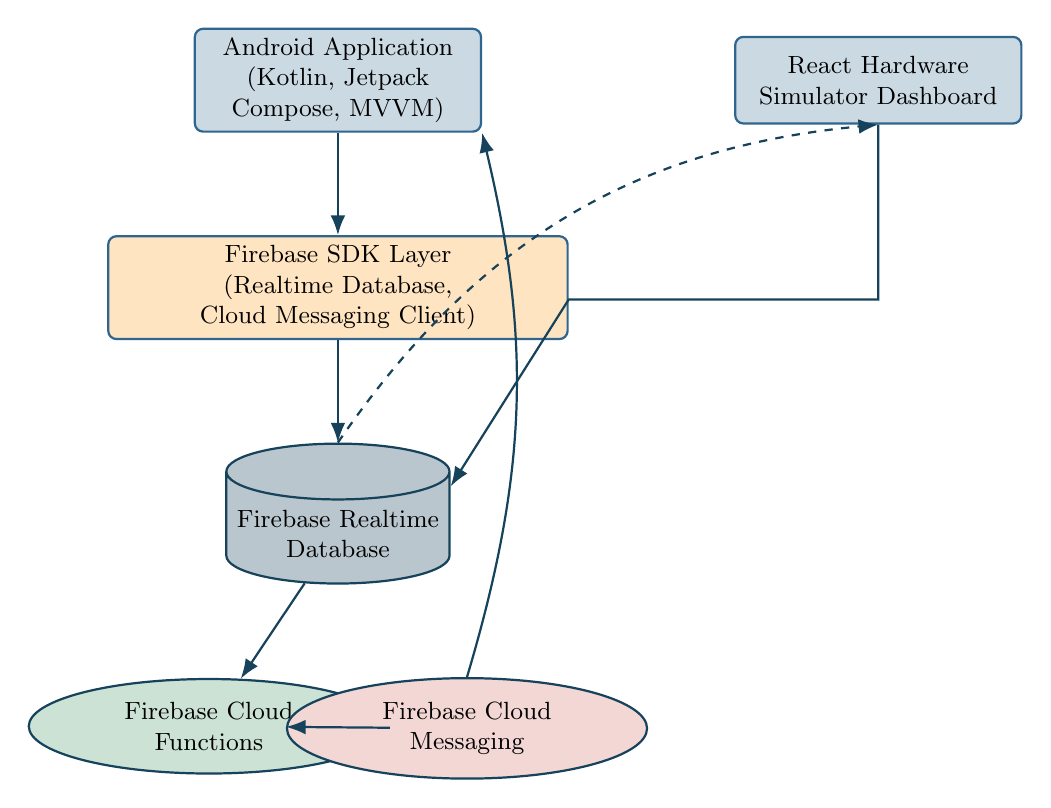
\begin{tikzpicture}[node distance=1.3cm and 2.2cm]

\node[block, fill=lumaprimary!25] (android) {Android Application\\(Kotlin, Jetpack Compose, MVVM)};
\node[blockwide, below=of android, fill=lumaaccent!30] (sdk) {Firebase SDK Layer\\(Realtime Database, Cloud Messaging Client)};
\node[dbnode, below=of sdk, fill=lumasecondary!30, text=black] (rtdb) {Firebase Realtime Database};
\node[block, right=3.2cm of android, fill=lumaprimary!25] (react) {React Hardware Simulator Dashboard};

\node[cloudnode, below left=1.4cm and -0.6cm of rtdb, fill=lumaok!25] (functions) {Firebase Cloud Functions};
\node[cloudnode, below right=1.4cm and -0.6cm of rtdb, fill=lumaerr!20] (fcm) {Firebase Cloud Messaging};

\draw[arrow] (android) -- (sdk);
\draw[arrow] (sdk) -- (rtdb);
\draw[arrow] (react.south) |- ($(sdk.east)+(0,-0.15)$) -- ($(rtdb.east)+(0,0.6)$);
\draw[arrow] (rtdb) -- (functions);
\draw[arrow] (functions) -- (fcm);
\draw[arrow] (fcm.north) to[bend right=15] (android.south east);

\draw[-{Latex[length=2.5mm]}, thick, lumasecondary, dashed] (rtdb.north) to[bend left=25] (react.south);

\end{tikzpicture}
\caption{High-level system architecture of Luma showing the Android application, the Firebase backend, and the React Hardware Simulator as independent clients of a shared Realtime Database.}
\label{fig:high-level-arch}
\end{figure}

\noindent The dashed arrow indicates that state changes written by the Hardware Simulator into the Realtime Database are pushed back out to the Android application (and vice versa) through Firebase's realtime listener mechanism, without either client ever contacting the other directly.

\subsection{Layered Architecture View}
Figure~\ref{fig:layered-arch} presents the same system as a layered stack, emphasizing the separation between the presentation layer, the synchronization layer, the cloud data layer, and the automation layer.

\begin{figure}[H]
\centering
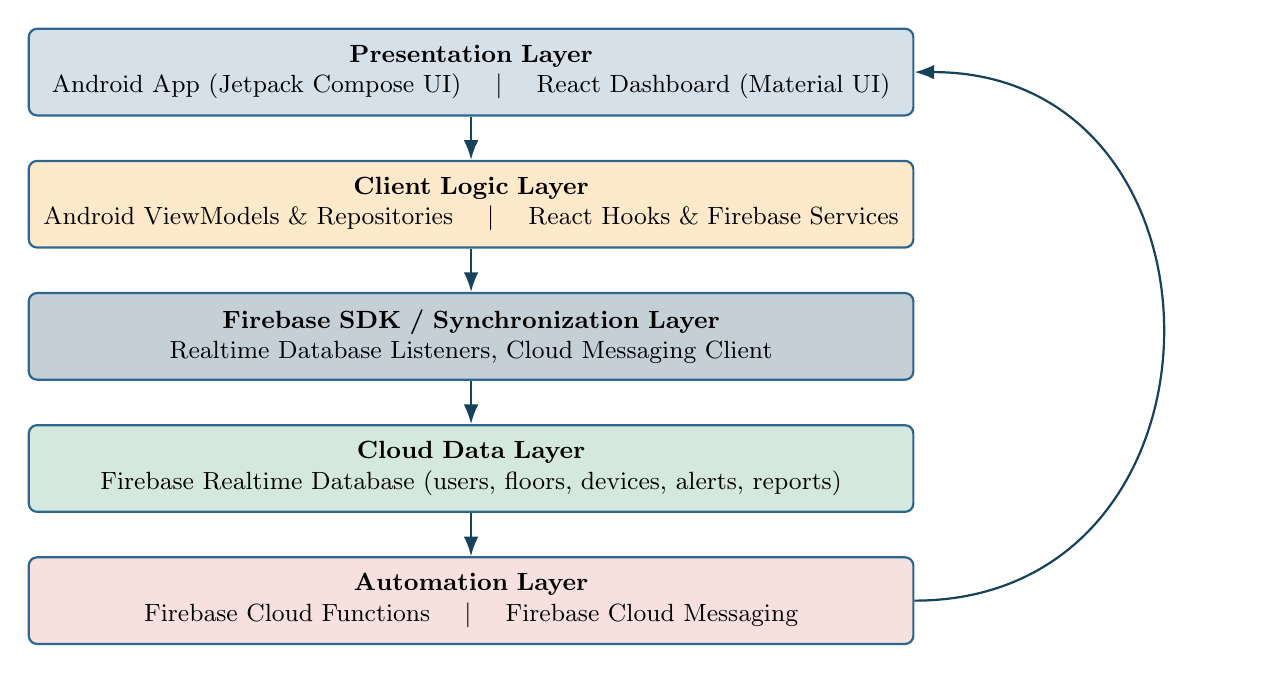
\begin{tikzpicture}[node distance=0.55cm]
\node[blockwide, minimum width=11cm, text width=11cm, fill=lumaprimary!20] (l1)
  {\textbf{Presentation Layer}\\ Android App (Jetpack Compose UI) \quad $\vert$ \quad React Dashboard (Material UI)};
\node[blockwide, minimum width=11cm, text width=11cm, below=of l1, fill=lumaaccent!25] (l2)
  {\textbf{Client Logic Layer}\\ Android ViewModels \& Repositories \quad $\vert$ \quad React Hooks \& Firebase Services};
\node[blockwide, minimum width=11cm, text width=11cm, below=of l2, fill=lumasecondary!25] (l3)
  {\textbf{Firebase SDK / Synchronization Layer}\\ Realtime Database Listeners, Cloud Messaging Client};
\node[blockwide, minimum width=11cm, text width=11cm, below=of l3, fill=lumaok!20] (l4)
  {\textbf{Cloud Data Layer}\\ Firebase Realtime Database (users, floors, devices, alerts, reports)};
\node[blockwide, minimum width=11cm, text width=11cm, below=of l4, fill=lumaerr!15] (l5)
  {\textbf{Automation Layer}\\ Firebase Cloud Functions \quad $\vert$ \quad Firebase Cloud Messaging};

\draw[arrow] (l1) -- (l2);
\draw[arrow] (l2) -- (l3);
\draw[arrow] (l3) -- (l4);
\draw[arrow] (l4) -- (l5);
\draw[-{Latex[length=2.5mm]}, thick, lumasecondary] (l5.east) to[out=0,in=0,looseness=1.6] (l1.east);
\end{tikzpicture}
\caption{Layered view of the Luma architecture, from user-facing presentation down to backend automation.}
\label{fig:layered-arch}
\end{figure}

\subsection{Component Responsibilities}

\begin{longtable}{@{}p{3.2cm}p{10.8cm}@{}}
\toprule
\textbf{Component} & \textbf{Responsibility} \\
\midrule
\endhead
Android Application & Presents floors, rooms, and devices to the homeowner; allows control actions; displays reports and notifications; observes the Realtime Database for live updates. \\
Firebase SDK & Provides the client libraries used by both the Android app and the React dashboard to read, write, and subscribe to changes in the Realtime Database, and to register for Cloud Messaging. \\
Firebase Realtime Database & Stores the canonical state of the entire home (floors, rooms, devices, alerts, reports) as a JSON tree; pushes incremental updates to all subscribed clients in real time. \\
Firebase Cloud Functions & Executes server-side logic in response to database writes -- for example, monitoring how long an electric iron has been switched on and automatically turning it off after the configured maximum duration. \\
Firebase Cloud Messaging & Delivers push notifications to the Android application when Cloud Functions detect safety-relevant events (e.g. automatic shutdown, device disconnection, device error). \\
React Hardware Simulator & A standalone web application that emulates the physical behaviour of smart devices (lights, outlets, switch panels, irons, cameras), writing simulated sensor and state data into the Realtime Database exactly as real hardware would. \\
\bottomrule
\caption{Responsibilities of each architectural component.}
\label{tab:component-responsibilities}
\end{longtable}

\subsection{Why Firebase Alone Is Sufficient}
A common design question is whether Luma requires a custom backend (for example, built with FastAPI, Node.js/Express, Spring Boot, or Django) in addition to Firebase. The team deliberately decided against this for the following reasons:

\begin{enumerate}[label=(\alph*)]
    \item \textbf{Realtime Database already provides the required data layer.} All entities in Luma (floors, rooms, devices, alerts, reports) are naturally represented as a JSON tree, which is exactly the data model that the Firebase Realtime Database is optimized for. A relational or document database behind a custom API would add complexity without adding capability.
    \item \textbf{Cloud Functions replace the need for a REST API.} The only server-side logic Luma requires -- automatic iron shutdown, alert generation, and report aggregation -- is naturally expressed as a reaction to a database write. Firebase Cloud Functions support exactly this trigger-based execution model, removing the need to design, host, and secure a separate REST API.
    \item \textbf{Built-in realtime synchronization.} A custom backend would require the team to implement WebSockets or a polling mechanism to achieve the same live-update behaviour that the Firebase Realtime Database provides out of the box.
    \item \textbf{Reduced operational overhead.} Firebase is a fully managed service; there is no server to provision, patch, or scale. This is particularly appropriate for a mini project with a fixed, short development timeline and no dedicated DevOps resource.
    \item \textbf{Built-in security rules.} Firebase Security Rules provide declarative, per-node access control directly on the database, removing the need to implement authentication and authorization middleware in a custom API layer.
    \item \textbf{Cost and simplicity.} Firebase's free tier is more than sufficient for a mini project of this scale, whereas hosting a custom backend would introduce additional cost and configuration overhead with no corresponding benefit to the project's learning objectives.
\end{enumerate}

\noindent The trade-off of this decision is discussed further in Section~\ref{sec:techstack}: a Firebase-only architecture is less portable to a non-Google cloud provider and offers less flexibility for complex relational queries than a traditional backend would, but for the scope of Luma these limitations are outweighed by the benefits above.

% ============================================================
\section{Technology Stack}
\label{sec:techstack}

\subsection{Mobile Technologies}
\begin{longtable}{@{}p{2.6cm}p{5.4cm}p{5cm}@{}}
\toprule
\textbf{Technology} & \textbf{Advantages} & \textbf{Disadvantages / Trade-offs} \\
\midrule
\endhead
Kotlin & Official first-class language for Android; concise, null-safe syntax; full interoperability with existing Java libraries; strong coroutine support for asynchronous Firebase calls. & Slightly steeper learning curve than Java for developers unfamiliar with functional-style syntax. \\
Android Studio & Official Android IDE with integrated emulator, layout inspector, Firebase Assistant plug-in, and Gradle build management. & Resource-intensive; requires a reasonably powerful development machine. \\
Jetpack Compose & Declarative UI toolkit that reduces boilerplate compared to XML layouts; integrates cleanly with ViewModel state via \texttt{State} and \texttt{Flow}; enables rapid iteration on the Dashboard, Floor Plan, and Device screens. & Relatively newer toolkit; some third-party libraries still offer better support for the legacy View system. \\
MVVM Architecture & Clear separation of UI, state-holding, and data-access logic; recommended by Google for Compose applications; simplifies unit testing of business logic in isolation from the UI. & Requires additional boilerplate (ViewModel, UiState classes) for very simple screens. \\
\bottomrule
\caption{Mobile technology choices and their trade-offs.}
\label{tab:mobile-tech}
\end{longtable}

\subsection{Cloud Technologies}
\begin{longtable}{@{}p{3.6cm}p{5.2cm}p{4.2cm}@{}}
\toprule
\textbf{Technology} & \textbf{Advantages} & \textbf{Disadvantages / Trade-offs} \\
\midrule
\endhead
Firebase Realtime Database & Low-latency, JSON-tree realtime synchronization out of the box; simple SDK for both Android and JavaScript; ideal for frequently changing device state. & Limited support for complex relational queries compared to Cloud Firestore or SQL. \\
Firebase Cloud Functions & Event-driven, serverless execution triggered directly by database writes; removes the need for a custom REST API or server hosting. & Cold-start latency on the free tier; execution time limits on long-running tasks. \\
Firebase Cloud Messaging & Reliable, Google-managed push notification delivery to Android devices, including when the app is in the background. & Requires correct handling of notification permissions on Android 13+. \\
Firebase Authentication (Optional) & Provides ready-made email/password and Google sign-in flows, tightly integrated with Realtime Database Security Rules. & Adds a dependency the mini project can optionally omit if a single shared household account is acceptable for demonstration purposes. \\
\bottomrule
\caption{Cloud technology choices and their trade-offs.}
\label{tab:cloud-tech}
\end{longtable}

\subsection{Web Dashboard Technologies}
\begin{longtable}{@{}p{2.6cm}p{5.4cm}p{5cm}@{}}
\toprule
\textbf{Technology} & \textbf{Advantages} & \textbf{Disadvantages / Trade-offs} \\
\midrule
\endhead
React & Component-based architecture maps naturally onto device cards, floor lists, and status chips; large ecosystem of hooks for Firebase integration. & Requires careful state management as the number of simulated devices grows. \\
Vite & Extremely fast development server and hot module replacement, well suited for rapid iteration on the simulator UI during testing. & Smaller plug-in ecosystem than older bundlers such as Webpack, though sufficient for this project's needs. \\
Material UI & Ready-made, accessible component library (cards, chips, switches, app bars) that accelerates dashboard construction and produces a professional look with minimal custom CSS. & Visual style can appear generic unless themed; theming was applied to match the Luma brand palette. \\
\bottomrule
\caption{Web dashboard technology choices and their trade-offs.}
\label{tab:web-tech}
\end{longtable}

\subsection{Version Control and Deployment}
\begin{longtable}{@{}p{3.6cm}p{5.2cm}p{4.2cm}@{}}
\toprule
\textbf{Technology} & \textbf{Advantages} & \textbf{Disadvantages / Trade-offs} \\
\midrule
\endhead
Git & Industry-standard distributed version control; enables the three-member team to work in parallel on Android, Firebase, and React codebases. & Requires discipline around branching and merge conflict resolution. \\
GitHub & Central remote repository, issue tracking, and pull-request based code review for the team. & None significant for a project of this scale. \\
Firebase Hosting & Free, HTTPS-enabled static hosting that integrates naturally with the rest of the Firebase project, ideal for deploying the React Hardware Simulator Dashboard. & Limited to static/serverless hosting; not required for this project since Cloud Functions cover backend logic. \\
Vercel (Alternative) & Zero-configuration deployment for React/Vite projects with automatic preview deployments per pull request. & Introduces a second cloud provider alongside Firebase; the team ultimately preferred Firebase Hosting for a single-provider deployment story. \\
\bottomrule
\caption{Version control and deployment options considered.}
\label{tab:devops-tech}
\end{longtable}

\subsection{Rejected Alternatives}
The team explicitly considered and rejected the following approaches:
\begin{itemize}
    \item \textbf{FastAPI / Node.js (Express) / Spring Boot / Django backend.} A custom REST API would duplicate functionality already provided by Firebase Realtime Database and Cloud Functions, while adding server hosting, authentication middleware, and API versioning overhead with no corresponding benefit for a project of this scope.
    \item \textbf{Cloud Firestore instead of Realtime Database.} Firestore offers richer querying but has higher per-write latency characteristics for very frequent small updates (such as a device toggling state many times during a demonstration); the simple JSON-tree model of the Realtime Database better matches Luma's data shape.
    \item \textbf{Native Android Views (XML layouts) instead of Jetpack Compose.} Compose was selected for its declarative model, which reduces boilerplate and pairs naturally with ViewModel-driven state in an MVVM architecture.
\end{itemize}

% ============================================================
\section{Project Folder Structures}
\label{sec:folderstructure}

\subsection{Android Application Folder Structure}
Figure~\ref{fig:android-folders} shows the package structure of the Android application, and Table~\ref{tab:android-folders-explained} explains the purpose of each package.

\begin{figure}[H]
\centering
\fcolorbox{lumaprimary}{codebg}{%
\begin{minipage}{0.7\linewidth}
\ttfamily\small
app/\\
\hspace*{1.2em}ui/\\
\hspace*{2.4em}dashboard/\\
\hspace*{2.4em}floor/\\
\hspace*{2.4em}device/\\
\hspace*{2.4em}report/\\
\hspace*{2.4em}settings/\\
\hspace*{1.2em}model/\\
\hspace*{1.2em}repository/\\
\hspace*{1.2em}firebase/\\
\hspace*{1.2em}viewmodel/\\
\hspace*{1.2em}navigation/\\
\hspace*{1.2em}utils/\\
\hspace*{1.2em}MainActivity.kt
\end{minipage}}
\caption{Android application package structure.}
\label{fig:android-folders}
\end{figure}

\begin{longtable}{@{}p{3.4cm}p{10.6cm}@{}}
\toprule
\textbf{Package} & \textbf{Purpose} \\
\midrule
\endhead
\texttt{ui/} & Root package for all Jetpack Compose UI code, organized by feature. \\
\texttt{ui/dashboard/} & Composables for the main Dashboard screen listing all floors. \\
\texttt{ui/floor/} & Composables for Floor List, Floor Details, and the interactive Floor Plan grid. \\
\texttt{ui/device/} & Composables for Device Details and Add Device screens, including per-device-type control widgets. \\
\texttt{ui/report/} & Composables for the Reports screen, including usage charts. \\
\texttt{ui/settings/} & Composables for the Settings screen. \\
\texttt{model/} & Kotlin data classes representing domain entities: \texttt{Floor}, \texttt{Room}, \texttt{Device}, \texttt{Alert}, \texttt{Report}, and device-specific subtypes. \\
\texttt{repository/} & Repository classes that abstract Firebase access behind a clean Kotlin API consumed by ViewModels, following the Repository pattern. \\
\texttt{firebase/} & Thin wrapper classes around the Firebase Realtime Database and Cloud Messaging SDKs, including listener registration and serialization helpers. \\
\texttt{viewmodel/} & ViewModel classes (one per screen/feature) that expose UI state as Kotlin \texttt{StateFlow} and handle user actions. \\
\texttt{navigation/} & Navigation graph definition using Jetpack Navigation Compose, including route definitions and argument passing. \\
\texttt{utils/} & Shared utility functions (date/time formatting, unit conversion, validation helpers). \\
\texttt{MainActivity.kt} & Application entry point; hosts the Compose \texttt{NavHost} and initializes Firebase. \\
\bottomrule
\caption{Explanation of Android application folders.}
\label{tab:android-folders-explained}
\end{longtable}

\subsection{React Hardware Simulator Folder Structure}
\begin{figure}[H]
\centering
\fcolorbox{lumaprimary}{codebg}{%
\begin{minipage}{0.6\linewidth}
\ttfamily\small
src/\\
\hspace*{1.2em}components/\\
\hspace*{1.2em}pages/\\
\hspace*{1.2em}firebase/\\
\hspace*{1.2em}hooks/\\
\hspace*{1.2em}utils/\\
\hspace*{1.2em}App.jsx\\
\hspace*{1.2em}main.jsx
\end{minipage}}
\caption{React Hardware Simulator Dashboard folder structure.}
\label{fig:react-folders}
\end{figure}

\begin{longtable}{@{}p{3.4cm}p{10.6cm}@{}}
\toprule
\textbf{Folder / File} & \textbf{Purpose} \\
\midrule
\endhead
\texttt{components/} & Reusable presentational components: Sidebar, Navbar, Device Card, Status Chip, Toggle Button, Floor Selector. \\
\texttt{pages/} & Top-level route components: Floor Overview page, Device Detail page, Camera Feed page. \\
\texttt{firebase/} & Firebase configuration and thin service functions for reading/writing device state to the Realtime Database. \\
\texttt{hooks/} & Custom React hooks (e.g. \texttt{useDeviceState}, \texttt{useFloorList}) that subscribe to Realtime Database listeners and expose live data to components. \\
\texttt{utils/} & Formatting and simulation-logic helpers, such as generating mock camera snapshots or simulated sensor jitter. \\
\texttt{App.jsx} & Root application component defining the overall dashboard layout and routing. \\
\texttt{main.jsx} & Vite/React entry point that mounts \texttt{App.jsx} into the DOM. \\
\bottomrule
\caption{Explanation of React Hardware Simulator folders.}
\label{tab:react-folders-explained}
\end{longtable}

% ============================================================
\section{Functional Requirements}
\label{sec:functional}

\subsection{Dashboard Requirements}
The Dashboard is the first substantive screen the user sees after the Splash Screen. It lists every floor currently defined for the home and allows floor-level management.

\begin{itemize}
    \item \textbf{View all floors.} The Dashboard displays a scrollable list/grid of floor cards, each showing the floor name, a thumbnail icon, the number of rooms, and a summary count of devices that are currently ON.
    \item \textbf{Add floor.} A floating action button opens a dialog in which the user enters a floor name (e.g. ``Ground Floor'', ``First Floor'') and selects an icon; on confirmation, a new floor node is created in the Realtime Database.
    \item \textbf{Delete floor.} A long-press or overflow menu on a floor card opens a confirmation dialog; on confirmation, the floor node and all of its child rooms/devices are removed from the database.
    \item \textbf{Edit floor.} The user can rename a floor or change its icon through the same dialog used for adding a floor, pre-populated with the existing values.
    \item \textbf{Select floor.} Tapping a floor card navigates to the Floor Details screen for that floor.
\end{itemize}

Figure~\ref{fig:wireframe-dashboard} shows a wireframe of the Dashboard screen.

\begin{figure}[H]
\centering
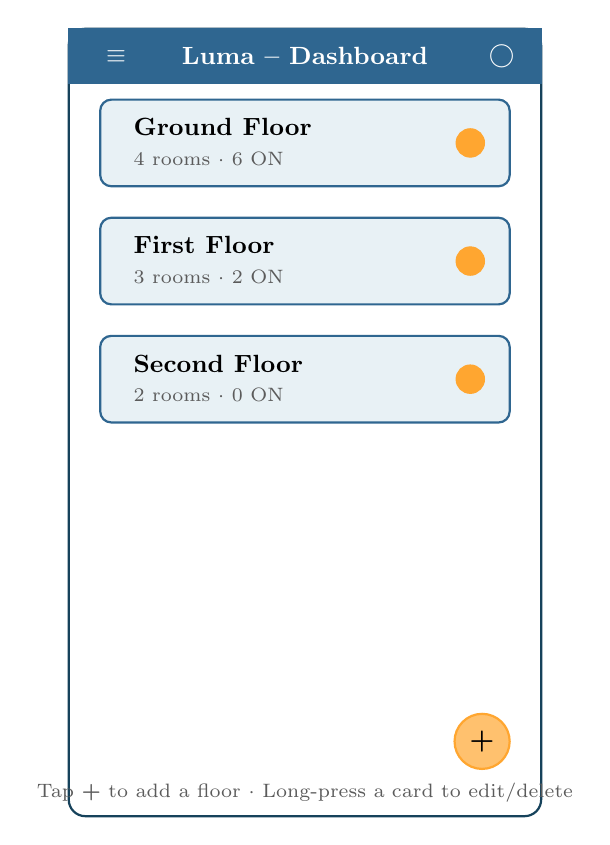
\begin{tikzpicture}[scale=1]
\draw[thick, lumasecondary, rounded corners=6pt] (0,0) rectangle (6,10);
\filldraw[lumaprimary] (0,9.3) rectangle (6,10);
\node[white, font=\bfseries\small] at (3,9.65) {Luma -- Dashboard};
\node[white, font=\small] at (0.6,9.65) {\(\equiv\)};
\node[white, font=\small] at (5.5,9.65) {\(\bigcirc\)};

\foreach \y/\name/\count in {8.0/Ground Floor/{4 rooms $\cdot$ 6 ON},6.5/First Floor/{3 rooms $\cdot$ 2 ON},5.0/Second Floor/{2 rooms $\cdot$ 0 ON}}{
  \draw[thick, lumaprimary, rounded corners=4pt, fill=lumalight] (0.4,\y) rectangle (5.6,\y+1.1);
  \node[font=\bfseries\small, anchor=west] at (0.7,\y+0.75) {\name};
  \node[font=\scriptsize, anchor=west, text=lumagray] at (0.7,\y+0.35) {\count};
  \draw[lumaaccent, fill=lumaaccent] (5.1,\y+0.55) circle (0.18);
}

\draw[thick, lumaaccent, fill=lumaaccent!70, rounded corners=10pt] (4.9,0.6) rectangle (5.6,1.3);
\node[font=\bfseries] at (5.25,0.95) {+};
\node[font=\scriptsize, text=lumagray] at (3,0.3) {Tap \textbf{+} to add a floor $\cdot$ Long-press a card to edit/delete};
\end{tikzpicture}
\caption{Wireframe of the Android Dashboard screen showing the floor list.}
\label{fig:wireframe-dashboard}
\end{figure}

\subsection{Floor Management}
Each floor contains one or more rooms, and each room contains one or more devices. The Floor Details screen presents rooms as an interactive grid, and selecting a room opens an interactive floor plan.

\begin{itemize}
    \item \textbf{Rooms.} Rooms are simple named containers (e.g. ``Living Room'', ``Kitchen'', ``Master Bedroom'') belonging to a floor.
    \item \textbf{Devices.} Each room contains zero or more devices, each with a type (outlet, light, switch panel, iron, camera), a name, and a current state.
    \item \textbf{Grid layout.} Rooms are displayed using a responsive grid (\texttt{LazyVerticalGrid} in Jetpack Compose) so that the number of visible room cards adapts to screen size.
    \item \textbf{Interactive floor plan.} Selecting a room opens a simplified 2D floor-plan view where devices are represented as tappable icons positioned approximately where they are physically located in the room, giving the user spatial context in addition to the flat device list.
\end{itemize}

\textbf{Implementation notes.} The Floor Details ViewModel subscribes to the \texttt{/floors/\{floorId\}/rooms} node of the Realtime Database. Each room composable further subscribes to \texttt{/floors/\{floorId\}/rooms/\{roomId\}/devices} so that device state changes are reflected immediately without requiring the user to refresh the screen. The floor-plan coordinates for each device are stored as normalized \texttt{x}, \texttt{y} fields (0.0--1.0) on the device record so that the layout scales correctly to any screen size.

% ============================================================
\section{Device Types and States}
\label{sec:devices}

Luma supports five categories of simulated smart devices. Each device type is modelled as a Kotlin sealed class on the Android side and as a corresponding JavaScript object shape on the React Hardware Simulator side, sharing a common JSON representation in the Realtime Database.

\subsection{Electrical Outlet}
\begin{itemize}
    \item \textbf{ON / OFF.} A single toggle switch controls whether the outlet is supplying power.
    \item \textbf{Realtime synchronization.} Toggling the outlet from either the Android app or the Hardware Simulator updates the \texttt{state} field of the device node, and the change propagates to all connected clients within the Realtime Database's typical sub-second latency.
\end{itemize}
The Electrical Outlet is the simplest device type in Luma and serves as the baseline example for the ON/OFF control pattern reused, in extended form, by the other device types.

\subsection{Smart Light}
\begin{itemize}
    \item \textbf{ON / OFF.} Manual toggle control, identical in behaviour to the Electrical Outlet.
    \item \textbf{Automatic scheduling.} The user can define a \texttt{startTime} and \texttt{endTime} (stored as HH:mm strings) after which a Cloud Function automatically turns the light on and off, simulating a timer-based automation rule.
    \item \textbf{Usage tracking.} Every ON$\to$OFF transition is appended to the device's \texttt{history} node with a timestamp, enabling the Reports feature (Section~\ref{sec:reports}) to compute total running time for the light.
\end{itemize}

\subsection{Multi-Switch Panel}
\begin{itemize}
    \item \textbf{Configurable switch count.} A single Multi-Switch Panel device can be configured with 2, 3, or 5 individual switches, matching common physical wall-panel form factors.
    \item \textbf{Independent control.} Each switch within the panel has its own \texttt{state} field (ON/OFF) and can be toggled independently of the others; the panel as a whole has no single combined state.
    \item \textbf{Data representation.} Switches are stored as a keyed sub-map (\texttt{switch1}, \texttt{switch2}, \ldots) under the panel's device node, as shown in Section~\ref{sec:database}.
\end{itemize}

\subsection{Electric Iron}
\begin{itemize}
    \item \textbf{ON / OFF.} Manual toggle control initiates or ends an ironing session.
    \item \textbf{Maximum operating duration.} A configurable maximum duration (default 30 minutes) defines the longest period the iron may remain switched on continuously, reflecting the fire-safety rationale for this feature.
    \item \textbf{Automatic shutdown.} A Firebase Cloud Function (detailed in Section~\ref{sec:cloudfunctions}) monitors the elapsed time since the iron was turned on and force-sets its state to OFF once the maximum duration is exceeded.
    \item \textbf{Push notification.} When the automatic shutdown occurs, a Cloud Function triggers a Firebase Cloud Messaging notification informing the user that the iron was switched off automatically for safety.
    \item \textbf{Realtime synchronization.} As with all devices, the resulting OFF state is immediately visible on both the Android app and the Hardware Simulator.
\end{itemize}
The Electric Iron is the primary demonstration of Luma's \emph{Safety Automation} objective (Section~\ref{sec:objectives}).

\subsection{Camera}
\begin{itemize}
    \item \textbf{Snapshot.} The user can request a still image representing the camera's current view.
    \item \textbf{Mock image.} Because no physical camera exists, the Hardware Simulator returns a pre-defined mock image (or a procedurally generated placeholder) rather than a live video feed.
    \item \textbf{Refresh image.} The Android app can request a new snapshot at any time, which updates the \texttt{lastSnapshotUrl} and \texttt{lastSnapshotAt} fields on the device node.
    \item \textbf{Connectivity states.} A camera device additionally exposes \texttt{online}, \texttt{offline}, and \texttt{disconnected} states, distinct from the simple ON/OFF model used by the other device types, since a camera's usefulness depends primarily on its connectivity rather than a power toggle.
\end{itemize}

\subsection{Device States}
Every device in Luma, regardless of type, exposes a \texttt{status} field in addition to its type-specific \texttt{state} fields. Table~\ref{tab:device-states} defines the possible values of this field and when each occurs.

\begin{longtable}{@{}p{2.6cm}p{10.6cm}@{}}
\toprule
\textbf{State} & \textbf{When It Occurs} \\
\midrule
\endhead
\texttt{ON} & The device (or, for a Multi-Switch Panel, an individual switch) is actively powered/active, either because the user switched it on manually, a schedule activated it, or a Cloud Function turned it on. \\
\texttt{OFF} & The device is intentionally powered down, either through manual user action, the end of a schedule, or an automatic safety shutdown (e.g. the Electric Iron's maximum-duration rule). \\
\texttt{ERROR} & The Hardware Simulator has flagged the device as reporting an invalid or unexpected internal condition (for example, simulated sensor failure); the Android app surfaces this with a red status chip and generates an alert. \\
\texttt{DISCONNECTED} & The device has not written a heartbeat/state update within the expected interval, simulating a device that has lost network connectivity; this state is periodically evaluated by a Cloud Function that compares the device's \texttt{lastSeen} timestamp against the current time. \\
\bottomrule
\caption{Device states and the conditions under which each occurs.}
\label{tab:device-states}
\end{longtable}

% ============================================================
\section{Usage Reports}
\label{sec:reports}

The Reports feature aggregates the \texttt{history} sub-nodes maintained for every device into summaries that help the user understand how the home is being used.

\subsection{Report Types}
\begin{itemize}
    \item \textbf{Daily Usage.} Total ON duration per device for the current calendar day, refreshed as new history entries arrive.
    \item \textbf{Weekly Usage.} Total ON duration per device, aggregated over the last seven days, useful for spotting week-over-week trends.
    \item \textbf{Monthly Usage.} Total ON duration per device, aggregated over the current calendar month.
    \item \textbf{Running Time.} The cumulative number of hours a given device has been active, since installation or since a user-selected reset point.
    \item \textbf{Power Usage.} An estimated energy consumption figure (kWh) computed by multiplying running time by a configurable nominal wattage per device type.
    \item \textbf{Safety Events.} A log of automatic-shutdown and disconnection events (e.g. iron auto-off events, device disconnections), each with a timestamp and the device involved.
\end{itemize}

\subsection{Report Visualizations}
Bar charts are used to compare running time across devices within a room or floor, while pie charts are used to show the proportional contribution of each device to total power usage. Figures~\ref{fig:report-bar} and~\ref{fig:report-pie} show representative examples of the intended chart styles.

\begin{figure}[H]
\centering
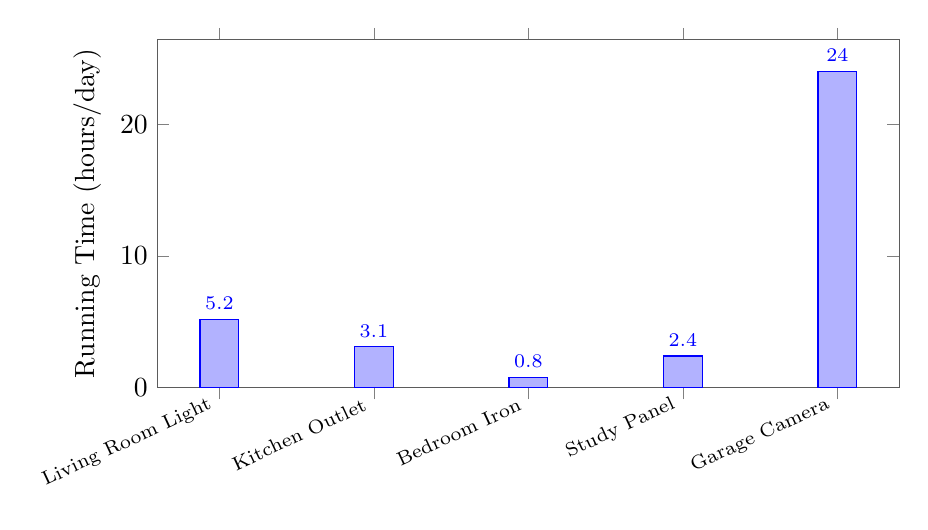
\begin{tikzpicture}
\begin{axis}[
    ybar, bar width=14pt,
    width=11cm, height=6cm,
    ylabel={Running Time (hours/day)},
    symbolic x coords={Living Room Light, Kitchen Outlet, Bedroom Iron, Study Panel, Garage Camera},
    xtick=data,
    x tick label style={rotate=25, anchor=east, font=\scriptsize},
    nodes near coords,
    nodes near coords style={font=\scriptsize},
    ymin=0,
    bar shift=0pt,
    axis line style={lumagray},
    every axis plot/.append style={fill=lumaprimary, draw=lumasecondary},
]
\addplot coordinates {
  (Living Room Light,5.2) (Kitchen Outlet,3.1) (Bedroom Iron,0.8) (Study Panel,2.4) (Garage Camera,24.0)
};
\end{axis}
\end{tikzpicture}
\caption{Example bar chart of daily device running time, as shown on the Reports screen.}
\label{fig:report-bar}
\end{figure}

\begin{figure}[H]
\centering
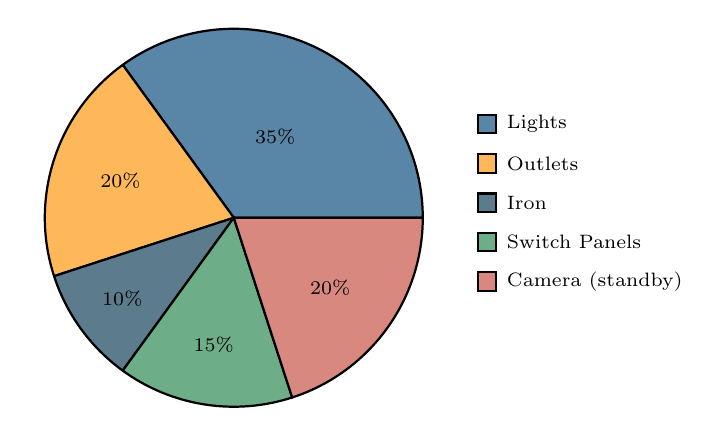
\begin{tikzpicture}
\pie[
  radius=2.4,
  text=legend,
  color={lumaprimary!80, lumaaccent!80, lumasecondary!70, lumaok!70, lumaerr!60},
  font=\scriptsize
]{
  35/Lights,
  20/Outlets,
  10/Iron,
  15/Switch Panels,
  20/Camera (standby)
}
\end{tikzpicture}
\caption{Example pie chart of proportional monthly power usage by device category.}
\label{fig:report-pie}
\end{figure}

\textbf{Implementation note.} The pie chart in Figure~\ref{fig:report-pie} is illustrative of the intended chart type; the production Android implementation renders equivalent bar and pie charts natively using a Compose charting library, with data sourced from the \texttt{ReportViewModel}, which aggregates the \texttt{/reports} node described in Section~\ref{sec:database}.

% ============================================================
\section{Notifications}
\label{sec:notifications}

Notifications keep the user informed of safety-relevant and connectivity-relevant events without requiring them to keep the app open.

\subsection{Notification Triggers}
\begin{itemize}
    \item \textbf{Iron automatically turned OFF.} Raised when the maximum-operating-duration Cloud Function forces an Electric Iron to OFF (Section~\ref{sec:cloudfunctions}).
    \item \textbf{Device disconnected.} Raised when a scheduled Cloud Function detects that a device's \texttt{lastSeen} timestamp has exceeded the disconnection threshold (default 60 seconds in the simulated environment).
    \item \textbf{Device error.} Raised when the Hardware Simulator writes an \texttt{ERROR} status for a device, simulating an internal fault.
\end{itemize}

\subsection{Delivery Mechanism}
\begin{itemize}
    \item \textbf{Cloud notification.} All notification triggers first write a structured entry into the \texttt{/alerts} node of the Realtime Database, giving the Android app an in-app notification history even if the device was offline when the event occurred.
    \item \textbf{Push notification.} In parallel, the Cloud Function that detected the event calls the Firebase Cloud Messaging Admin SDK to deliver a push notification to the registered device token(s) for the household, ensuring the user is alerted even when the Android app is in the background or closed.
\end{itemize}

Figure~\ref{fig:notification-flow} illustrates the notification pipeline for the iron auto-shutdown scenario, which is representative of all three trigger types.

\begin{figure}[H]
\centering
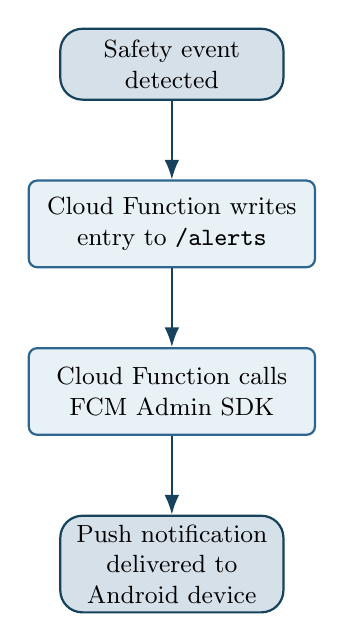
\begin{tikzpicture}[node distance=1cm]
\node[startstop] (event) {Safety event detected};
\node[block, below=of event] (write) {Cloud Function writes entry to \texttt{/alerts}};
\node[block, below=of write] (fcm) {Cloud Function calls FCM Admin SDK};
\node[startstop, below=of fcm] (push) {Push notification delivered to Android device};
\draw[arrow] (event) -- (write);
\draw[arrow] (write) -- (fcm);
\draw[arrow] (fcm) -- (push);
\end{tikzpicture}
\caption{Notification delivery pipeline shared by all three notification triggers.}
\label{fig:notification-flow}
\end{figure}

% ============================================================
\section{Hardware Simulator Dashboard}
\label{sec:simulator}

\subsection{Purpose}
The Hardware Simulator Dashboard is a completely separate React web application; it is \textbf{not} part of the Android application and is not distributed to the end user. Its sole purpose is to stand in for physical IoT hardware during development and demonstration, by writing realistic, time-varying state data into the same Firebase Realtime Database that the Android application reads from. From the perspective of the Realtime Database and the Cloud Functions, data written by the simulator is indistinguishable from data that would be written by real hardware, which allows the rest of the system to be developed and evaluated as if physical devices were present.

\subsection{Simulation Behaviour}
\begin{itemize}
    \item Each simulated device periodically writes a \texttt{lastSeen} heartbeat timestamp, allowing the disconnection-detection Cloud Function to be exercised realistically.
    \item Toggling a device card in the simulator writes directly to the corresponding device's \texttt{state} field, exactly as the Android app does, demonstrating bidirectional synchronization.
    \item The simulator can be manually instructed (via a developer control) to simulate a device entering the \texttt{ERROR} or \texttt{DISCONNECTED} state, to test the Android app's handling of these states without waiting for a real fault.
    \item The Camera device type returns a mock image on snapshot request rather than a live feed, consistent with the absence of real camera hardware.
\end{itemize}

\subsection{Dashboard Layout}
Figure~\ref{fig:wireframe-simulator} shows a wireframe of the Hardware Simulator Dashboard layout.

\begin{figure}[H]
\centering
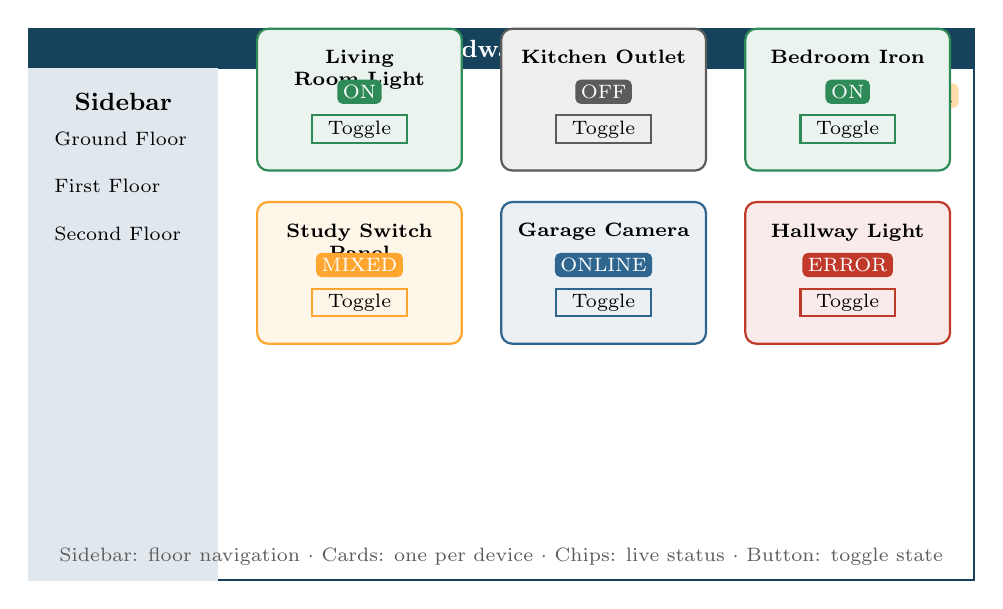
\begin{tikzpicture}[scale=1]
\draw[thick, lumasecondary] (0,0) rectangle (12,7);
\filldraw[lumasecondary] (0,6.5) rectangle (12,7);
\node[white, font=\bfseries\small] at (6,6.75) {Luma Hardware Simulator};

\filldraw[lumaprimary!15] (0,0) rectangle (2.4,6.5);
\node[font=\bfseries\small, anchor=north] at (1.2,6.3) {Sidebar};
\foreach \y/\name in {5.6/Ground Floor,5.0/First Floor,4.4/Second Floor}{
  \node[font=\scriptsize, anchor=west] at (0.2,\y) {\name};
}

\node[font=\scriptsize, fill=lumaaccent!40, rounded corners=2pt, inner sep=2pt] at (10.6,6.15) {Status: Connected};

\foreach \x/\y/\name/\state/\col in {2.9/5.2/Living Room Light/ON/lumaok,6.0/5.2/Kitchen Outlet/OFF/lumagray,9.1/5.2/Bedroom Iron/ON/lumaok,2.9/3.0/Study Switch Panel/MIXED/lumaaccent,6.0/3.0/Garage Camera/ONLINE/lumaprimary,9.1/3.0/Hallway Light/ERROR/lumaerr}{
  \draw[thick, \col, rounded corners=4pt, fill=\col!10] (\x,\y) rectangle (\x+2.6,\y+1.8);
  \node[font=\bfseries\scriptsize, anchor=north, text width=2.4cm, align=center] at (\x+1.3,\y+1.65) {\name};
  \node[font=\scriptsize, fill=\col, text=white, rounded corners=2pt, inner sep=2pt] at (\x+1.3,\y+1.0) {\state};
  \draw[thick, \col] (\x+0.7,\y+0.35) rectangle (\x+1.9,\y+0.7);
  \node[font=\scriptsize] at (\x+1.3,\y+0.525) {Toggle};
}
\node[font=\scriptsize, text=lumagray] at (6,0.3) {Sidebar: floor navigation $\cdot$ Cards: one per device $\cdot$ Chips: live status $\cdot$ Button: toggle state};
\end{tikzpicture}
\caption{Wireframe of the React Hardware Simulator Dashboard.}
\label{fig:wireframe-simulator}
\end{figure}

\noindent The layout consists of a \textbf{Navbar} across the top showing the simulator title and Firebase connection status, a \textbf{Sidebar} listing floors for navigation, a main content area of \textbf{Device Cards} (one per device) each showing a \textbf{Status Chip} reflecting the current device state and a \textbf{Toggle Button} for manual control, and a live realtime-update indicator confirming that the dashboard is subscribed to the Realtime Database.

% ============================================================
\section{Firebase Database Design}
\label{sec:database}

\subsection{Database Structure Overview}
The Realtime Database is organized as a single JSON tree with five top-level nodes: \texttt{users}, \texttt{floors}, \texttt{devices}, \texttt{alerts}, and \texttt{reports}. Devices are stored in a flat top-level node (rather than nested inside floors/rooms) and referenced by ID from within the floor/room structure, which is a deliberate denormalization that keeps individual device listeners lightweight, following Firebase's recommended best practice of flattening deeply nested data.

\begin{figure}[H]
\centering
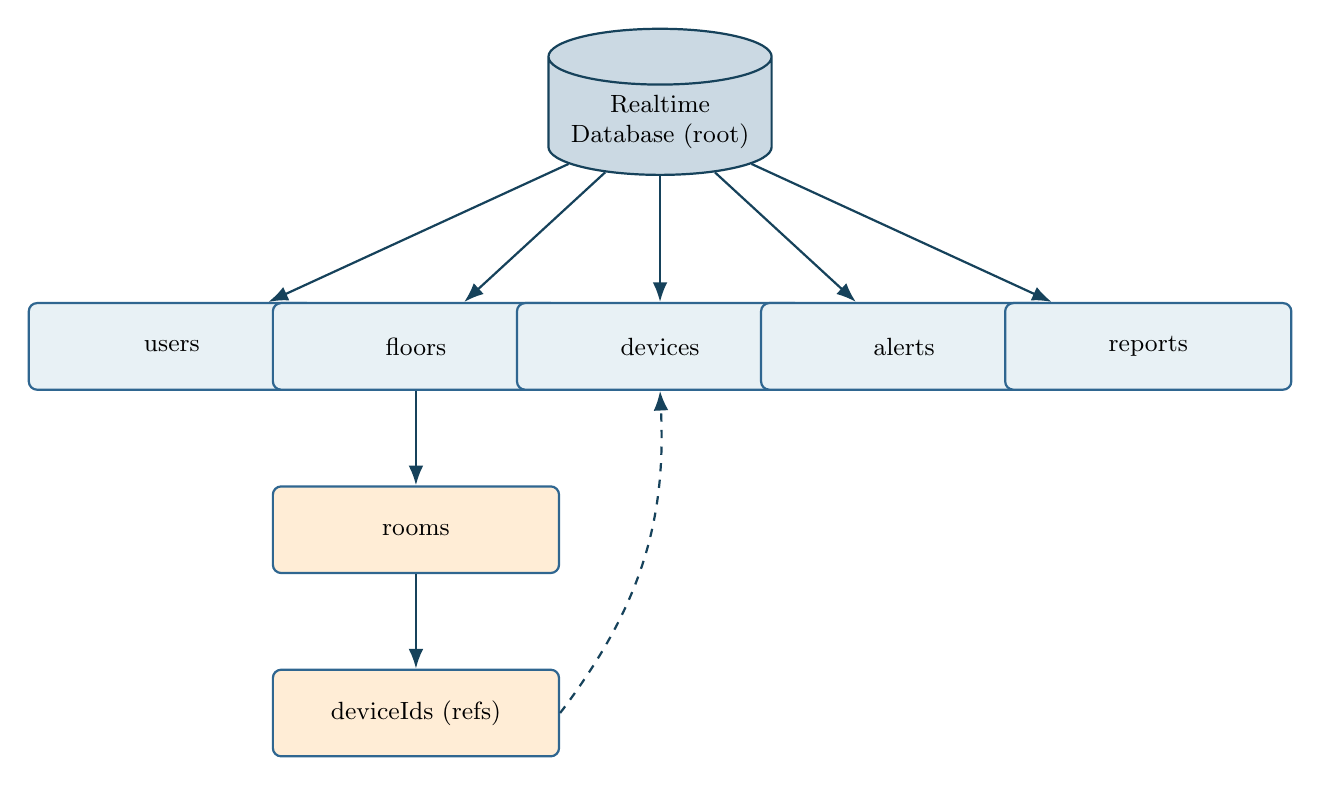
\begin{tikzpicture}[node distance=1.1cm and 2.6cm]
\node[dbnode, fill=lumaprimary!25, text=black] (root) {Realtime Database (root)};
\node[block, below=1.6cm of root, xshift=-6.2cm] (users) {users};
\node[block, below=1.6cm of root, xshift=-3.1cm] (floors) {floors};
\node[block, below=1.6cm of root] (devices) {devices};
\node[block, below=1.6cm of root, xshift=3.1cm] (alerts) {alerts};
\node[block, below=1.6cm of root, xshift=6.2cm] (reports) {reports};

\draw[arrow] (root) -- (users);
\draw[arrow] (root) -- (floors);
\draw[arrow] (root) -- (devices);
\draw[arrow] (root) -- (alerts);
\draw[arrow] (root) -- (reports);

\node[block, below=1.2cm of floors, fill=lumaaccent!20] (rooms) {rooms};
\draw[arrow] (floors) -- (rooms);
\node[block, below=1.2cm of rooms, fill=lumaaccent!20] (deviceids) {deviceIds (refs)};
\draw[arrow] (rooms) -- (deviceids);
\draw[-{Latex[length=2.5mm]}, thick, lumasecondary, dashed] (deviceids.east) to[bend right=20] (devices.south);
\end{tikzpicture}
\caption{Top-level Firebase Realtime Database structure. Dashed arrow indicates a reference (device ID) rather than nested ownership.}
\label{fig:db-structure}
\end{figure}

\subsection{Entity-Relationship Diagram}
Although the Realtime Database is non-relational, the logical relationships between entities are best understood through the ER-style diagram in Figure~\ref{fig:er-diagram}.

\begin{figure}[H]
\centering
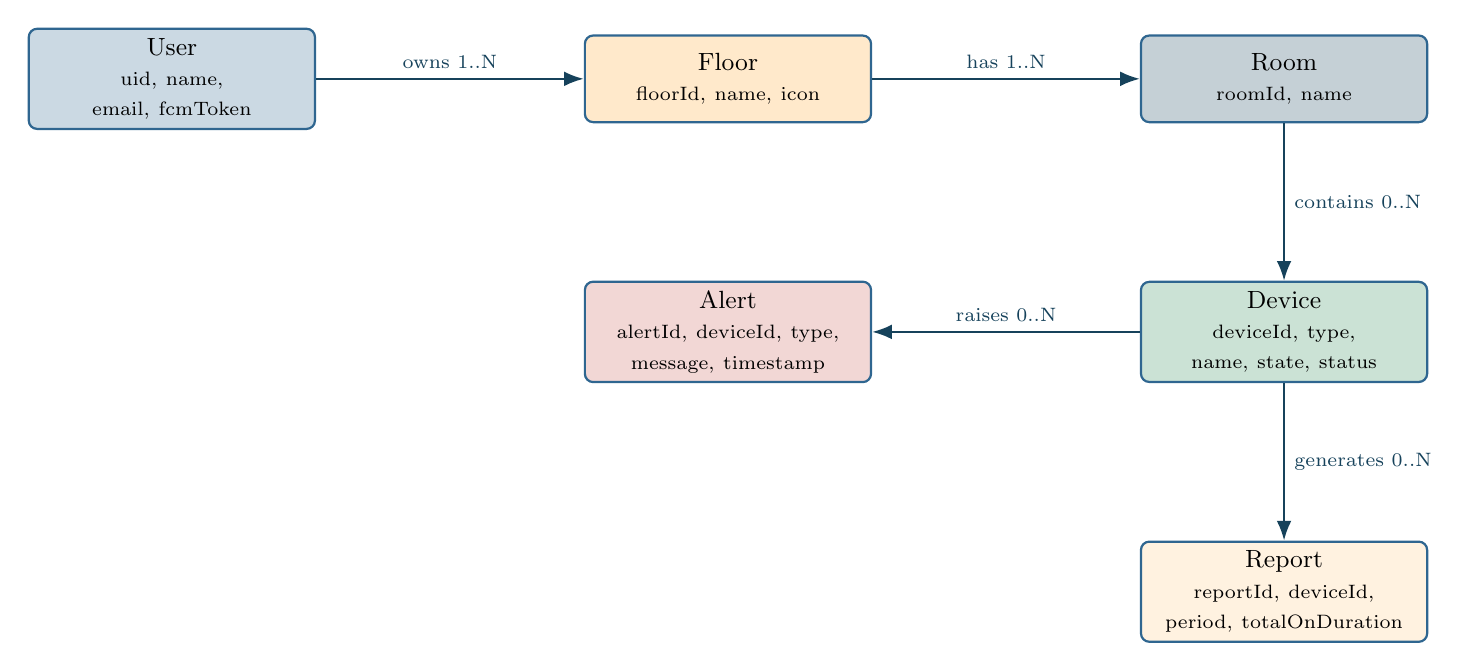
\begin{tikzpicture}[node distance=2.0cm]
\node[block, fill=lumaprimary!25] (user) {User\\\scriptsize uid, name, email, fcmToken};
\node[block, right=3.4cm of user, fill=lumaaccent!25] (floor) {Floor\\\scriptsize floorId, name, icon};
\node[block, right=3.4cm of floor, fill=lumasecondary!25] (room) {Room\\\scriptsize roomId, name};
\node[block, below=2.0cm of room, fill=lumaok!25] (device) {Device\\\scriptsize deviceId, type, name, state, status};
\node[block, left=3.4cm of device, fill=lumaerr!20] (alert) {Alert\\\scriptsize alertId, deviceId, type, message, timestamp};
\node[block, below=2.0cm of device, fill=lumaaccent!15] (report) {Report\\\scriptsize reportId, deviceId, period, totalOnDuration};

\draw[arrow] (user) -- node[above,font=\scriptsize]{owns 1..N} (floor);
\draw[arrow] (floor) -- node[above,font=\scriptsize]{has 1..N} (room);
\draw[arrow] (room) -- node[right,font=\scriptsize]{contains 0..N} (device);
\draw[arrow] (device) -- node[above,font=\scriptsize]{raises 0..N} (alert);
\draw[arrow] (device) -- node[right,font=\scriptsize]{generates 0..N} (report);
\end{tikzpicture}
\caption{Entity-Relationship diagram of the Luma data model.}
\label{fig:er-diagram}
\end{figure}

\subsection{JSON Schema Examples}

\begin{lstlisting}[language=json,caption={Example JSON structure for a single floor with one room and a device reference.},label={lst:json-floor}]
"floors": {
  "floor001": {
    "name": "Ground Floor",
    "icon": "home",
    "rooms": {
      "room001": {
        "name": "Living Room",
        "devices": {
          "device001": true,
          "device002": true
        }
      }
    }
  }
}
\end{lstlisting}

\begin{lstlisting}[language=json,caption={Example JSON structure for devices, including an Electric Iron and a Multi-Switch Panel.},label={lst:json-devices}]
"devices": {
  "device001": {
    "type": "iron",
    "name": "Bedroom Iron",
    "state": "ON",
    "status": "ON",
    "turnedOnAt": 1739000000000,
    "maxDurationMinutes": 30,
    "lastSeen": 1739000590000
  },
  "device002": {
    "type": "switchPanel",
    "name": "Study Switch Panel",
    "switchCount": 3,
    "switches": {
      "switch1": "ON",
      "switch2": "OFF",
      "switch3": "OFF"
    },
    "status": "ON",
    "lastSeen": 1739000600000
  }
}
\end{lstlisting}

\begin{lstlisting}[language=json,caption={Example JSON structure for an alert and a report entry.},label={lst:json-alerts}]
"alerts": {
  "alert001": {
    "deviceId": "device001",
    "type": "AUTO_SHUTDOWN",
    "message": "Iron automatically turned OFF after 30 minutes",
    "timestamp": 1739001800000
  }
},
"reports": {
  "device001_2026-07-10": {
    "deviceId": "device001",
    "period": "daily",
    "date": "2026-07-10",
    "totalOnDurationMinutes": 48,
    "estimatedKwh": 0.6
  }
}
\end{lstlisting}

\subsection{Relationships Summary}
\begin{itemize}
    \item A \textbf{User} owns one or more \textbf{Floors} (a single-household deployment in this mini project owns all floors; multi-user support is discussed as a future improvement in Section~\ref{sec:future}).
    \item A \textbf{Floor} contains one or more \textbf{Rooms}.
    \item A \textbf{Room} contains zero or more \textbf{Devices}, referenced by ID rather than nested directly, keeping the \texttt{devices} node flat and each device's listener lightweight.
    \item A \textbf{Device} may raise zero or more \textbf{Alerts} over its lifetime.
    \item A \textbf{Device} generates one \textbf{Report} entry per aggregation period (daily/weekly/monthly).
\end{itemize}

% ============================================================
\section{Android Application Screens}
\label{sec:screens}

This section documents the ten primary screens of the Luma Android application. For each screen, the purpose, key components, navigation behaviour, expected behaviour, user interactions, and possible future improvements are described. Wireframes are provided for the most structurally significant screens; the Dashboard and Hardware Simulator wireframes were already presented in Figures~\ref{fig:wireframe-dashboard} and~\ref{fig:wireframe-simulator}.

\subsection{Splash Screen}
\textbf{Purpose.} Displays the Luma logo and tagline while Firebase initializes and an initial authentication/connectivity check is performed.\\
\textbf{Components.} Centered logo, tagline text, indeterminate progress indicator.\\
\textbf{Navigation.} Automatically navigates to the Dashboard after initialization completes (typically under one second); no back-navigation is possible from this screen.\\
\textbf{Expected behaviour.} If Firebase initialization fails (e.g. no network connectivity), an inline retry message is shown instead of navigating forward.\\
\textbf{User interactions.} None beyond an optional retry tap on failure.\\
\textbf{Future improvements.} Add an animated logo reveal and a persisted-session check to skip directly to a previously selected floor.

\subsection{Dashboard}
\textbf{Purpose.} Entry point for floor-level monitoring and management, as detailed in Section~\ref{sec:functional}.\\
\textbf{Components.} Top app bar, scrollable floor card list, floating action button for adding a floor.\\
\textbf{Navigation.} Tapping a floor card navigates to Floor Details; the overflow menu in the app bar links to Settings and Notifications.\\
\textbf{Expected behaviour.} The floor list updates live as devices under any floor change state (e.g. the ``ON count'' badge on each card).\\
\textbf{User interactions.} Tap to select a floor, long-press or overflow-menu tap to edit/delete a floor, FAB tap to add a floor.\\
\textbf{Wireframe.} See Figure~\ref{fig:wireframe-dashboard}.\\
\textbf{Future improvements.} Add drag-to-reorder floors and a home-wide ``all devices off'' quick action.

\subsection{Floor List}
\textbf{Purpose.} An alternate, denser list view of all floors, accessible from the navigation drawer, intended for homes with many floors.\\
\textbf{Components.} Compact list rows (icon, name, room count), search/filter field.\\
\textbf{Navigation.} Tapping a row navigates to Floor Details for that floor.\\
\textbf{Expected behaviour.} Supports text filtering by floor name for fast access in larger homes.\\
\textbf{User interactions.} Tap to select, swipe to reveal quick edit/delete actions.\\
\textbf{Future improvements.} Add alphabetical/usage-based sorting options.

\subsection{Floor Details}
\textbf{Purpose.} Shows the rooms belonging to a selected floor in a responsive grid, per Section~\ref{sec:functional}.\\
\textbf{Components.} Floor name header, room grid (\texttt{LazyVerticalGrid}), per-room device-count badges.\\
\textbf{Navigation.} Tapping a room card navigates to the Floor Plan screen for that room; back navigation returns to the Dashboard.\\
\textbf{Expected behaviour.} Room cards update live to reflect the number of devices currently ON.\\
\textbf{User interactions.} Tap to open a room, overflow menu to add/rename/delete a room.\\
\textbf{Future improvements.} Add a floor-level ``all rooms off'' action and room reordering.

\subsection{Floor Plan}
\textbf{Purpose.} Provides an interactive 2D spatial view of a room's devices, positioned according to their normalized \texttt{x}/\texttt{y} coordinates, as described in Section~\ref{sec:functional}.\\
\textbf{Components.} Simplified room outline, device icons positioned on the plan, tap targets for each device.\\
\textbf{Navigation.} Tapping a device icon navigates to Device Details.\\
\textbf{Expected behaviour.} Device icons visually reflect current state (e.g. a light icon glows amber when ON).\\
\textbf{User interactions.} Tap a device to view details; drag-and-drop (in edit mode) to reposition a device on the plan.\\
\textbf{Future improvements.} Support importing a real floor-plan image as the background layer.

\subsection{Device Details}
\textbf{Purpose.} Displays full status and controls for a single device, with a layout that adapts to the device's type (Section~\ref{sec:devices}).\\
\textbf{Components.} Device name/type header, status chip, type-specific control widgets (toggle, per-switch toggles, schedule picker, snapshot button), a mini history/usage summary.\\
\textbf{Navigation.} Back navigation returns to the Floor Plan or Floor Details screen depending on entry point.\\
\textbf{Expected behaviour.} Control actions write directly to the Realtime Database and the UI reflects the resulting state change as soon as the listener fires, typically within a fraction of a second.\\
\textbf{User interactions.} Toggle ON/OFF, adjust schedule times (Smart Light), toggle individual switches (Multi-Switch Panel), request snapshot (Camera), rename or remove the device.\\
\textbf{Future improvements.} Add per-device notification preferences and a live sparkline of recent state changes.

\subsection{Add Device}
\textbf{Purpose.} Allows the user to register a new (simulated) device within a room.\\
\textbf{Components.} Device type selector, name field, room/floor confirmation, type-specific configuration fields (e.g. switch count for a Multi-Switch Panel, maximum duration for an Electric Iron).\\
\textbf{Navigation.} Presented as a modal/full-screen dialog over Floor Plan or Floor Details; dismiss or save returns to the calling screen.\\
\textbf{Expected behaviour.} On save, a new device node is created under \texttt{/devices} and referenced from the selected room.\\
\textbf{User interactions.} Select device type, fill configuration fields, tap Save or Cancel.\\
\textbf{Future improvements.} Add device templates and bulk-add for Multi-Switch Panels.

\subsection{Reports}
\textbf{Purpose.} Presents daily, weekly, and monthly usage summaries as described in Section~\ref{sec:reports}.\\
\textbf{Components.} Period selector (Daily/Weekly/Monthly), bar chart of running time, pie chart of power usage proportion, safety-events list.\\
\textbf{Navigation.} Accessible from the Dashboard app bar; back navigation returns to the Dashboard.\\
\textbf{Expected behaviour.} Charts re-render when the selected period changes or when new history data arrives.\\
\textbf{User interactions.} Switch report period, tap a chart segment to drill into a specific device's history.\\
\textbf{Future improvements.} Add CSV/PDF export and year-over-year comparison views.

\subsection{Notifications}
\textbf{Purpose.} Displays the in-app history of alerts described in Section~\ref{sec:notifications}.\\
\textbf{Components.} Chronological list of alert cards (icon, message, timestamp, affected device link).\\
\textbf{Navigation.} Tapping an alert navigates to the relevant Device Details screen.\\
\textbf{Expected behaviour.} New alerts appear at the top of the list in real time as they are written to \texttt{/alerts}.\\
\textbf{User interactions.} Tap to view the related device, swipe to dismiss/mark as read.\\
\textbf{Future improvements.} Add per-category notification filtering and mute/snooze controls.

\subsection{Settings}
\textbf{Purpose.} Exposes application-level preferences.\\
\textbf{Components.} Notification toggle, theme (light/dark) selector, default iron maximum-duration preference, account/sign-out section (if Firebase Authentication is enabled), app version/about section.\\
\textbf{Navigation.} Accessible from the Dashboard app bar; back navigation returns to the Dashboard.\\
\textbf{Expected behaviour.} Preference changes are applied immediately and, where relevant, written to the user's profile node.\\
\textbf{User interactions.} Toggle switches, tap to open sub-dialogs (e.g. default duration picker).\\
\textbf{Future improvements.} Add per-household member permission management once multi-user support (Section~\ref{sec:future}) is introduced.

% ============================================================
\section{Navigation Flow}
\label{sec:navigation}

\subsection{Primary Navigation Path}
Figure~\ref{fig:nav-flow} shows the primary linear navigation path through the application, from launch to the deepest common screens.

\begin{figure}[H]
\centering
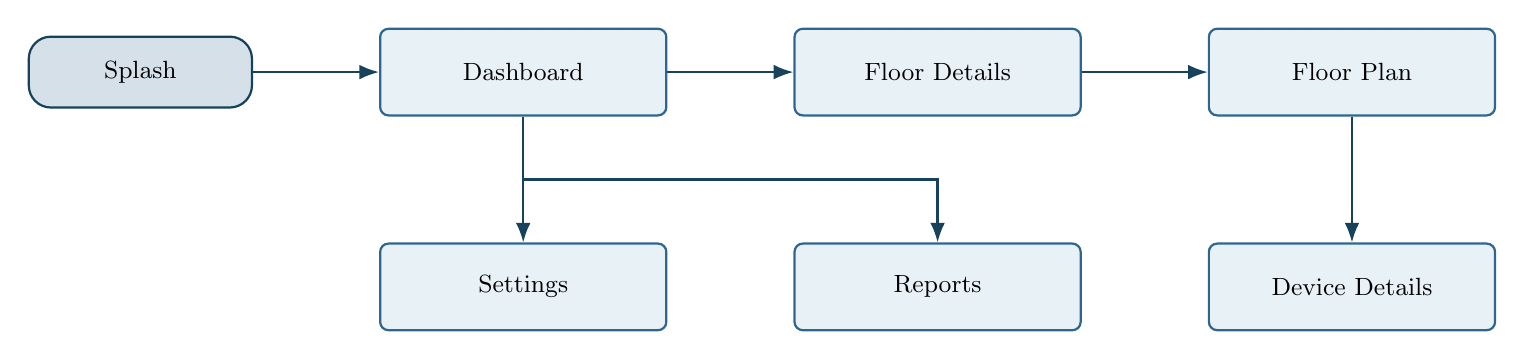
\begin{tikzpicture}[node distance=1.6cm]
\node[startstop] (splash) {Splash};
\node[block, right=of splash] (dashboard) {Dashboard};
\node[block, right=of dashboard] (floor) {Floor Details};
\node[block, right=of floor] (plan) {Floor Plan};
\node[block, below=1.6cm of plan] (device) {Device Details};
\node[block, left=of device] (reports) {Reports};
\node[block, left=of reports] (settings) {Settings};

\draw[arrow] (splash) -- (dashboard);
\draw[arrow] (dashboard) -- (floor);
\draw[arrow] (floor) -- (plan);
\draw[arrow] (plan) -- (device);
\draw[arrow] (dashboard.south) |- ++(0,-0.8) -| (reports.north);
\draw[arrow] (dashboard.south) |- ++(0,-1.1) -| (settings.north);
\end{tikzpicture}
\caption{Primary navigation flow of the Luma Android application.}
\label{fig:nav-flow}
\end{figure}

\subsection{Navigation Architecture}
Navigation is implemented using \textbf{Jetpack Navigation Compose}. A single \texttt{NavHost} is hosted in \texttt{MainActivity}, with each screen registered as a composable destination in the \texttt{navigation/} package (Section~\ref{sec:folderstructure}). Screens that require a parameter (Floor Details, Floor Plan, Device Details) receive it as a typed navigation argument (e.g. \texttt{floorId}, \texttt{roomId}, \texttt{deviceId}) encoded into the route string, which allows the corresponding ViewModel to be constructed with the correct Firebase path via a \texttt{SavedStateHandle}. The Dashboard, Reports, Settings, and Notifications screens are also reachable as top-level destinations from a persistent navigation drawer / bottom navigation bar, allowing the user to jump between these sections without returning to the Dashboard first.

\subsection{Use Case Diagram}
Figure~\ref{fig:use-case} presents the primary use cases available to the homeowner (the sole actor for this mini project, given that multi-user support is a future improvement).

\begin{figure}[H]
\centering
\begin{tikzpicture}
\node (actor) at (0,3) {\begin{tikzpicture}
\draw[thick] (0,0) circle (0.25);
\draw[thick] (0,-0.25) -- (0,-1.1);
\draw[thick] (-0.4,-0.6) -- (0.4,-0.6);
\draw[thick] (0,-1.1) -- (-0.35,-1.7);
\draw[thick] (0,-1.1) -- (0.35,-1.7);
\end{tikzpicture}};
\node[below=0.1cm of actor, font=\small] {Homeowner};

\draw[thick] (3.2,4.4) ellipse (10cm and 3.4cm);
\node[font=\bfseries\small] at (3.2,7.3) {Luma System};

\foreach \pos/\label in {
  {(0.6,5.8)}/{Monitor Devices},
  {(3.0,6.2)}/{Control Devices},
  {(6.0,5.8)}/{Manage Floors \& Rooms},
  {(0.6,4.4)}/{Add / Remove Device},
  {(3.0,4.4)}/{View Reports},
  {(6.0,4.4)}/{Receive Notifications},
  {(0.6,3.0)}/{Configure Schedule},
  {(3.0,2.6)}/{Simulate Device (Simulator)},
  {(6.0,3.0)}/{Adjust Settings}
}{
  \draw[thick, lumaprimary, fill=lumalight] \pos ellipse (1.55cm and 0.55cm);
  \node[font=\scriptsize, text width=2.6cm, align=center] at \pos {\label};
}

\draw[thick] (actor.east) -- (0.6,5.8);
\draw[thick] (actor.east) -- (3.0,6.2);
\draw[thick] (actor.east) -- (6.0,5.8);
\draw[thick] (actor.east) -- (0.6,4.4);
\draw[thick] (actor.east) -- (3.0,4.4);
\draw[thick] (actor.east) -- (6.0,4.4);
\draw[thick] (actor.east) -- (0.6,3.0);
\draw[thick] (actor.east) -- (6.0,3.0);
\end{tikzpicture}
\caption{Use case diagram for the Luma system, with the Homeowner as the primary actor. ``Simulate Device'' is exercised through the separate Hardware Simulator application during development and demonstration.}
\label{fig:use-case}
\end{figure}

\subsection{Sequence Diagram: Controlling a Device}
Figure~\ref{fig:sequence-diagram} shows the sequence of interactions when the user toggles a device from the Android application and the change propagates to the Hardware Simulator.

\begin{figure}[H]
\centering
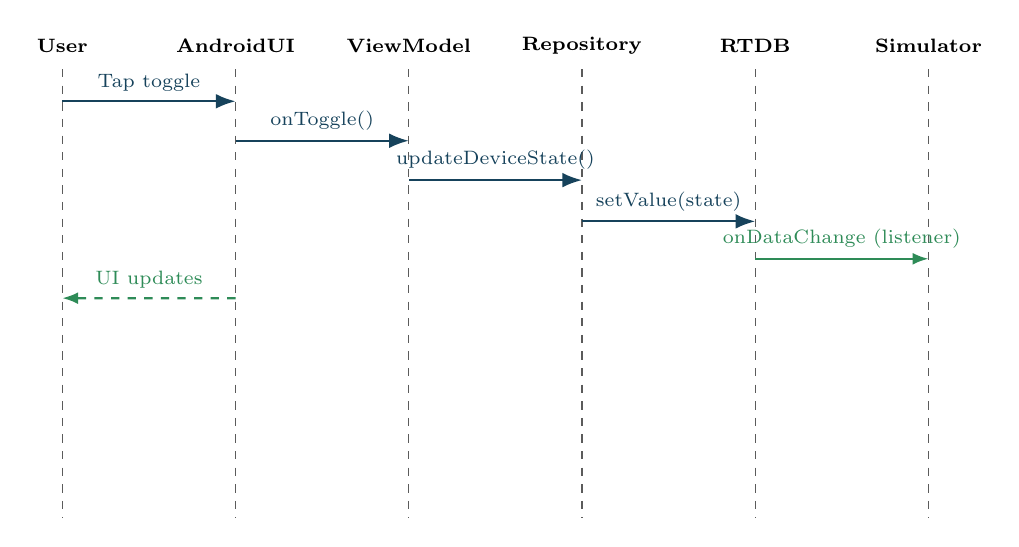
\begin{tikzpicture}[font=\scriptsize]
\node at (0,6) (h0) {\textbf{User}};
\node at (2.2,6) (h1) {\textbf{AndroidUI}};
\node at (4.4,6) (h2) {\textbf{ViewModel}};
\node at (6.6,6) (h3) {\textbf{Repository}};
\node at (8.8,6) (h4) {\textbf{RTDB}};
\node at (11.0,6) (h5) {\textbf{Simulator}};
\foreach \i in {0,1,2,3,4,5} {
  \draw[dashed, lumagray] (\i*2.2,5.7) -- (\i*2.2,0);
}
\draw[arrow] (h0.south) ++(0,-0.5) -- ++(2.2,0) node[midway,above]{Tap toggle};
\draw[arrow] (h1.south) ++(0,-1.0) -- ++(2.2,0) node[midway,above]{onToggle()};
\draw[arrow] (h2.south) ++(0,-1.5) -- ++(2.2,0) node[midway,above]{updateDeviceState()};
\draw[arrow] (h3.south) ++(0,-2.0) -- ++(2.2,0) node[midway,above]{setValue(state)};
\draw[-{Latex[length=2mm]}, thick, lumaok] (h4.south) ++(0,-2.5) -- ++(2.2,0) node[midway,above]{onDataChange (listener)};
\draw[-{Latex[length=2mm]}, thick, lumaok, dashed] ($(h1.south)+(0,-3.0)$) -- ($(h0.south)+(0,-3.0)$) node[midway,above]{UI updates};
\end{tikzpicture}
\caption{Sequence diagram for a device control action, from user tap through to the Hardware Simulator observing the resulting state change.}
\label{fig:sequence-diagram}
\end{figure}

\subsection{Activity Diagram: Electric Iron Safety Automation}
Figure~\ref{fig:activity-diagram} models the activity flow of the Electric Iron's automatic-shutdown safety feature, described functionally in Section~\ref{sec:devices} and implemented in Section~\ref{sec:cloudfunctions}.

\begin{figure}[H]
\centering
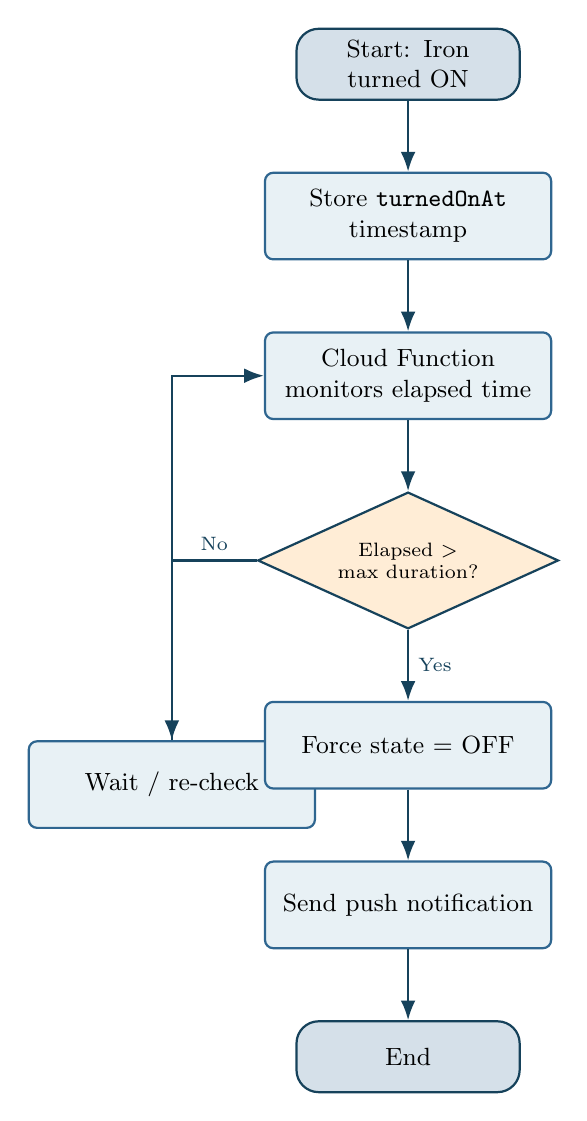
\begin{tikzpicture}[node distance=0.9cm]
\node[startstop] (start) {Start: Iron turned ON};
\node[block, below=of start] (store) {Store \texttt{turnedOnAt} timestamp};
\node[block, below=of store] (monitor) {Cloud Function monitors elapsed time};
\node[decision, below=of monitor] (check) {Elapsed \textgreater\ max duration?};
\node[block, below=1.4cm of check, xshift=-3.0cm] (wait) {Wait / re-check};
\node[block, below=of check] (shutoff) {Force state = OFF};
\node[block, below=of shutoff] (notify) {Send push notification};
\node[startstop, below=of notify] (end) {End};

\draw[arrow] (start) -- (store);
\draw[arrow] (store) -- (monitor);
\draw[arrow] (monitor) -- (check);
\draw[arrow] (check.west) -| node[near start, above, font=\scriptsize]{No} (wait.north);
\draw[arrow] (wait.north) |- ($(monitor.west)+(0,0)$);
\draw[arrow] (check) -- node[right, font=\scriptsize]{Yes} (shutoff);
\draw[arrow] (shutoff) -- (notify);
\draw[arrow] (notify) -- (end);
\end{tikzpicture}
\caption{Activity diagram for the Electric Iron automatic-shutdown safety feature.}
\label{fig:activity-diagram}
\end{figure}

\subsection{UML Class Diagram}
Figure~\ref{fig:class-diagram} shows a simplified class diagram of the core Android domain and data-access classes.

\begin{figure}[H]
\centering
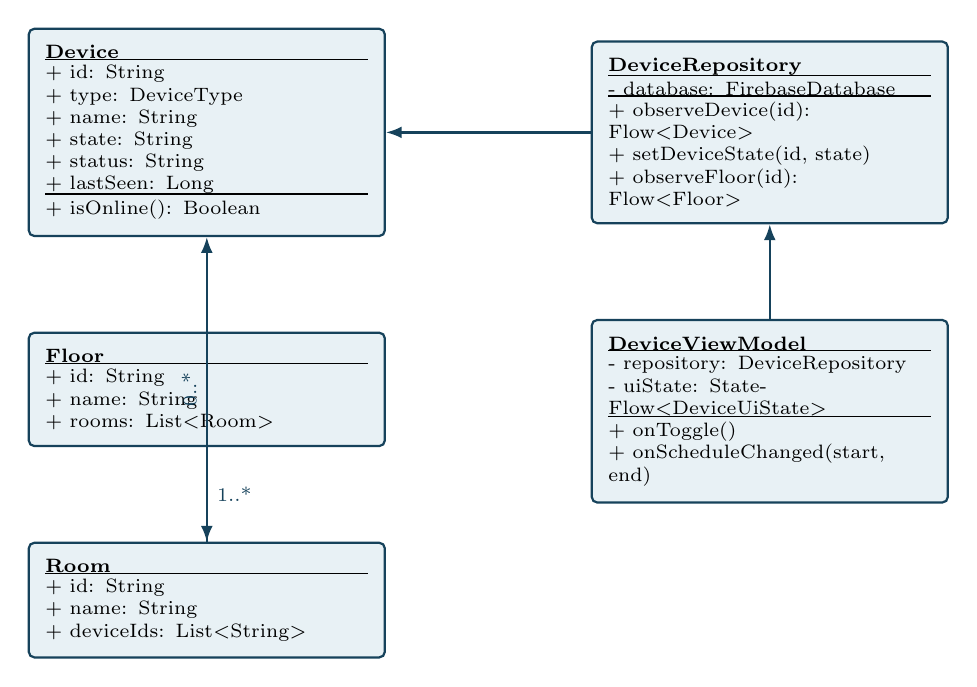
\begin{tikzpicture}[node distance=1.2cm and 1.4cm,
  classbox/.style={rectangle, draw=lumasecondary, thick, fill=lumalight, text width=4.1cm, align=left, font=\scriptsize, inner sep=6pt, rounded corners=2pt}]

\node[classbox] (device) {\textbf{Device}\\\hrule\vspace{2pt}
+ id: String\\ + type: DeviceType\\ + name: String\\ + state: String\\ + status: String\\ + lastSeen: Long\\\hrule\vspace{2pt}
+ isOnline(): Boolean};

\node[classbox, right=2.6cm of device] (repo) {\textbf{DeviceRepository}\\\hrule\vspace{2pt}
- database: FirebaseDatabase\\\hrule\vspace{2pt}
+ observeDevice(id): Flow\textless Device\textgreater\\
+ setDeviceState(id, state)\\
+ observeFloor(id): Flow\textless Floor\textgreater};

\node[classbox, below=of repo] (vm) {\textbf{DeviceViewModel}\\\hrule\vspace{2pt}
- repository: DeviceRepository\\ - uiState: StateFlow\textless DeviceUiState\textgreater\\\hrule\vspace{2pt}
+ onToggle()\\ + onScheduleChanged(start, end)};

\node[classbox, below=of device] (floor) {\textbf{Floor}\\\hrule\vspace{2pt}
+ id: String\\ + name: String\\ + rooms: List\textless Room\textgreater};

\node[classbox, below=of floor] (room) {\textbf{Room}\\\hrule\vspace{2pt}
+ id: String\\ + name: String\\ + deviceIds: List\textless String\textgreater};

\draw[-{Latex[length=2mm]}, thick, lumasecondary] (floor) -- node[right,font=\scriptsize]{1..*} (room);
\draw[-{Latex[length=2mm]}, thick, lumasecondary] (room) -- node[above,font=\scriptsize, sloped]{0..*} (device);
\draw[-{Latex[length=2mm]}, thick, lumasecondary] (repo) -- (device);
\draw[-{Latex[length=2mm]}, thick, lumasecondary] (vm) -- (repo);
\end{tikzpicture}
\caption{Simplified UML class diagram of the core Android domain and repository classes.}
\label{fig:class-diagram}
\end{figure}

% ============================================================
\section{Firebase Synchronization}
\label{sec:sync}

\subsection{Bidirectional Synchronization Model}
Because the Android application and the React Hardware Simulator never communicate directly, all synchronization is mediated by the Firebase Realtime Database's listener mechanism. Figure~\ref{fig:sync-android-to-dash} and Figure~\ref{fig:sync-dash-to-android} show the two symmetric synchronization paths.

\begin{figure}[H]
\centering
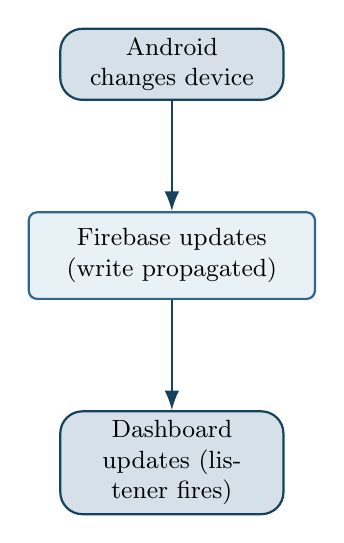
\begin{tikzpicture}[node distance=1.4cm]
\node[startstop] (a1) {Android changes device};
\node[block, below=of a1] (a2) {Firebase updates (write propagated)};
\node[startstop, below=of a2] (a3) {Dashboard updates (listener fires)};
\draw[arrow] (a1) -- (a2);
\draw[arrow] (a2) -- (a3);
\end{tikzpicture}
\caption{Synchronization path: Android application to Hardware Simulator Dashboard.}
\label{fig:sync-android-to-dash}
\end{figure}

\begin{figure}[H]
\centering
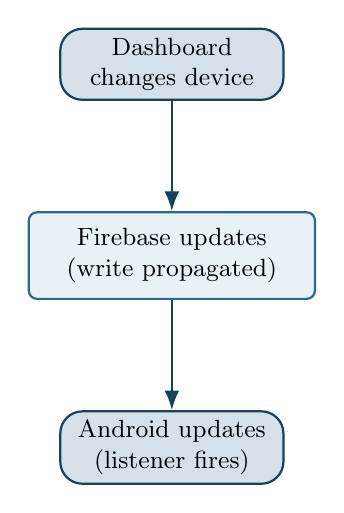
\begin{tikzpicture}[node distance=1.4cm]
\node[startstop] (b1) {Dashboard changes device};
\node[block, below=of b1] (b2) {Firebase updates (write propagated)};
\node[startstop, below=of b2] (b3) {Android updates (listener fires)};
\draw[arrow] (b1) -- (b2);
\draw[arrow] (b2) -- (b3);
\end{tikzpicture}
\caption{Synchronization path: Hardware Simulator Dashboard to Android application.}
\label{fig:sync-dash-to-android}
\end{figure}

\subsection{Realtime Database Listeners}
On Android, synchronization is implemented using the Firebase Realtime Database's \texttt{ValueEventListener} and \texttt{ChildEventListener} APIs, wrapped by the \texttt{DeviceRepository} class (Figure~\ref{fig:class-diagram}) into a Kotlin \texttt{Flow} using \texttt{callbackFlow}, so that ViewModels can consume updates using standard coroutine collection (\texttt{collectAsState} in Compose). On the React dashboard, the equivalent behaviour is achieved using the Firebase JavaScript SDK's \texttt{onValue} listener, wrapped inside custom hooks such as \texttt{useDeviceState}, which internally call \texttt{onValue} on mount and detach the listener with the returned unsubscribe function on unmount.

A listener is attached at the narrowest path that satisfies a given screen's needs -- for example, the Device Details screen listens only to \texttt{/devices/\{deviceId\}} rather than the entire \texttt{/devices} node -- to minimize bandwidth and re-render frequency.

\subsection{Consistency and Conflict Handling}
Because the Realtime Database applies writes in the order they are received per client connection and broadcasts the resulting value to all listeners, the system exhibits \emph{eventual consistency with last-write-wins} semantics at the level of an individual field. For Luma's use case -- a single household with, in practice, one active operator at a time -- this is an acceptable trade-off. Where atomicity across multiple fields is required (for example, when the iron auto-shutdown Cloud Function must simultaneously set \texttt{state} to OFF and clear \texttt{turnedOnAt}), the implementation uses Firebase's multi-path \texttt{update()} call, which is applied atomically across all specified paths.

% ============================================================
\section{Firebase Cloud Functions}
\label{sec:cloudfunctions}

\subsection{Role of Cloud Functions}
Firebase Cloud Functions provide the only server-side logic in Luma, executing in Google's managed Node.js runtime in response to Realtime Database triggers (\texttt{onValueWritten} / \texttt{onValueUpdated}) rather than in response to direct HTTP calls from either client. This event-driven model is what allows Luma to avoid a custom REST API entirely, as discussed in Section~\ref{sec:architecture}.

\subsection{Iron Automatic Shutdown Function}
The most safety-critical Cloud Function in Luma monitors every Electric Iron device for excessive continuous operation. Figure~\ref{fig:cloud-function-flow} shows the end-to-end flow, from the user switching the iron on through to all clients being updated.

\begin{figure}[H]
\centering
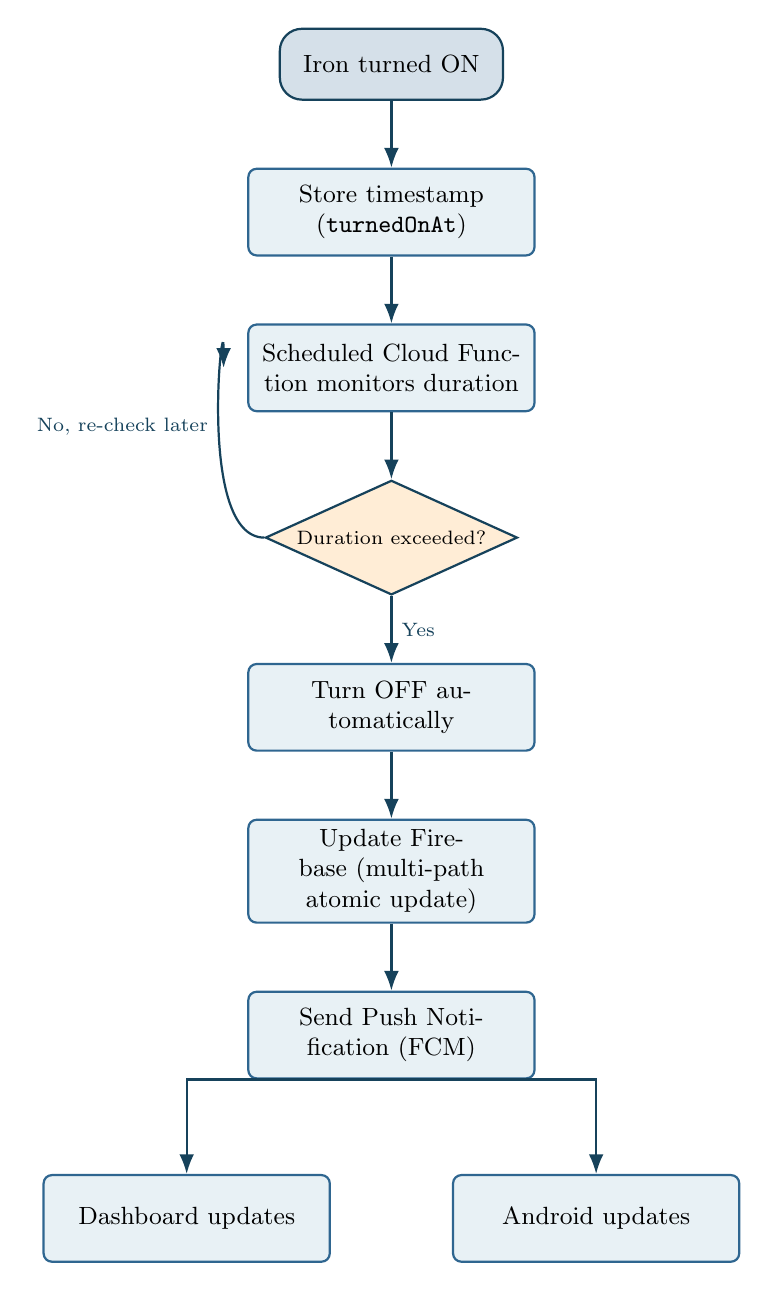
\begin{tikzpicture}[node distance=0.85cm]
\node[startstop] (n1) {Iron turned ON};
\node[block, below=of n1] (n2) {Store timestamp (\texttt{turnedOnAt})};
\node[block, below=of n2] (n3) {Scheduled Cloud Function monitors duration};
\node[decision, below=of n3] (n4) {Duration exceeded?};
\node[block, below=of n4] (n5) {Turn OFF automatically};
\node[block, below=of n5] (n6) {Update Firebase (multi-path atomic update)};
\node[block, below=of n6] (n7) {Send Push Notification (FCM)};
\node[block, below=1.2cm of n7, xshift=-2.6cm] (n8) {Dashboard updates};
\node[block, below=1.2cm of n7, xshift=2.6cm] (n9) {Android updates};

\draw[arrow] (n1) -- (n2);
\draw[arrow] (n2) -- (n3);
\draw[arrow] (n3) -- (n4);
\draw[arrow] (n4) -- node[right,font=\scriptsize]{Yes} (n5);
\draw[arrow] (n4.west) to[out=180,in=90] node[left,font=\scriptsize]{No, re-check later} ($(n3.west)+(-0.3,0)$);
\draw[arrow] (n5) -- (n6);
\draw[arrow] (n6) -- (n7);
\draw[arrow] (n7.south) -| (n8.north);
\draw[arrow] (n7.south) -| (n9.north);
\end{tikzpicture}
\caption{Flowchart of the Firebase Cloud Function implementing the Electric Iron automatic-shutdown safety feature.}
\label{fig:cloud-function-flow}
\end{figure}

\begin{lstlisting}[language=json,caption={Simplified pseudocode for the iron auto-shutdown Cloud Function.},label={lst:cloud-function-pseudo}]
exports.checkIronDuration = functions.pubsub
  .schedule("every 1 minutes")
  .onRun(async () => {
    const devices = await db.ref("devices").once("value");
    devices.forEach((snap) => {
      const d = snap.val();
      if (d.type === "iron" && d.state === "ON") {
        const elapsedMin = (Date.now() - d.turnedOnAt) / 60000;
        if (elapsedMin >= d.maxDurationMinutes) {
          db.ref(`devices/${snap.key}`).update({
            state: "OFF",
            status: "OFF",
            turnedOnAt: null
          });
          db.ref("alerts").push({
            deviceId: snap.key,
            type: "AUTO_SHUTDOWN",
            message: "Iron automatically turned OFF after " +
                     d.maxDurationMinutes + " minutes",
            timestamp: Date.now()
          });
          sendPushNotification(d.ownerFcmToken, snap.key);
        }
      }
    });
  });
\end{lstlisting}

\subsection{Other Cloud Functions}
\begin{itemize}
    \item \textbf{Disconnection Detector.} A scheduled function that periodically compares each device's \texttt{lastSeen} timestamp against the current time and marks the device as \texttt{DISCONNECTED} if the threshold is exceeded, raising an alert as described in Section~\ref{sec:notifications}.
    \item \textbf{Smart Light Scheduler.} A scheduled function that evaluates each Smart Light's configured \texttt{startTime}/\texttt{endTime} against the current time and toggles the light's state accordingly.
    \item \textbf{Report Aggregator.} A function triggered whenever a device's \texttt{history} node receives a new ON$\to$OFF entry, which recomputes the affected device's daily/weekly/monthly totals under \texttt{/reports}.
    \item \textbf{Alert Notifier.} A generic function triggered on any write to \texttt{/alerts} that forwards the alert to Firebase Cloud Messaging, used by both the disconnection detector and the iron auto-shutdown function.
\end{itemize}

% ============================================================
\section{MVVM Architecture}
\label{sec:mvvm}

\subsection{Overview}
The Android application follows the \textbf{Model-View-ViewModel (MVVM)} pattern, which is the architecture recommended by Google for Jetpack Compose applications. Figure~\ref{fig:mvvm-diagram} shows the flow of data and events through the four architectural layers used in Luma.

\begin{figure}[H]
\centering
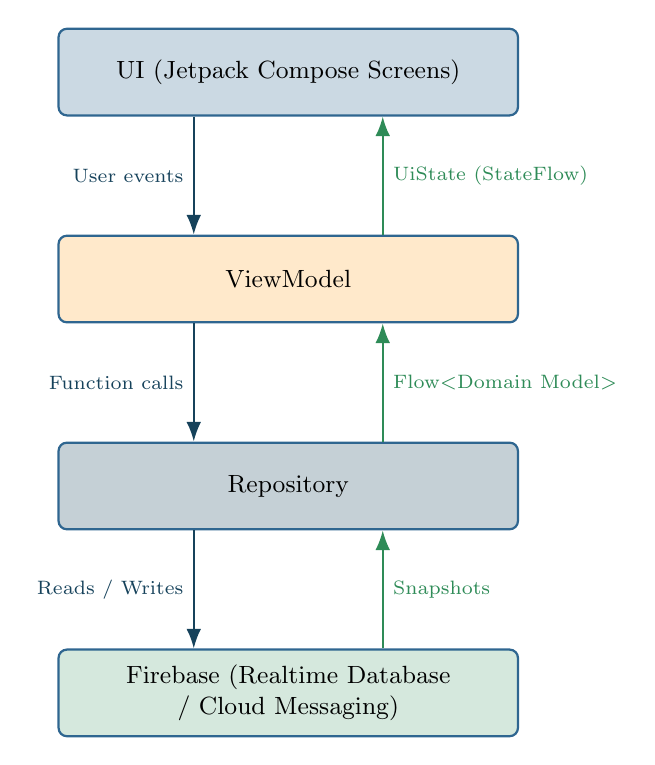
\begin{tikzpicture}[node distance=1.5cm]
\node[blockwide, fill=lumaprimary!25] (ui) {UI (Jetpack Compose Screens)};
\node[blockwide, below=of ui, fill=lumaaccent!25] (vm) {ViewModel};
\node[blockwide, below=of vm, fill=lumasecondary!25] (repo) {Repository};
\node[blockwide, below=of repo, fill=lumaok!20] (fb) {Firebase (Realtime Database / Cloud Messaging)};

\draw[-{Latex[length=2.5mm]}, thick, lumasecondary] ($(ui.south)+(-1.2,0)$) -- ($(vm.north)+(-1.2,0)$) node[midway, left, font=\scriptsize]{User events};
\draw[-{Latex[length=2.5mm]}, thick, lumaok] ($(vm.north)+(1.2,0)$) -- ($(ui.south)+(1.2,0)$) node[midway, right, font=\scriptsize]{UiState (StateFlow)};

\draw[-{Latex[length=2.5mm]}, thick, lumasecondary] ($(vm.south)+(-1.2,0)$) -- ($(repo.north)+(-1.2,0)$) node[midway, left, font=\scriptsize]{Function calls};
\draw[-{Latex[length=2.5mm]}, thick, lumaok] ($(repo.north)+(1.2,0)$) -- ($(vm.south)+(1.2,0)$) node[midway, right, font=\scriptsize]{Flow\textless Domain Model\textgreater};

\draw[-{Latex[length=2.5mm]}, thick, lumasecondary] ($(repo.south)+(-1.2,0)$) -- ($(fb.north)+(-1.2,0)$) node[midway, left, font=\scriptsize]{Reads / Writes};
\draw[-{Latex[length=2.5mm]}, thick, lumaok] ($(fb.north)+(1.2,0)$) -- ($(repo.south)+(1.2,0)$) node[midway, right, font=\scriptsize]{Snapshots}; 
\end{tikzpicture}
\caption{MVVM architecture as applied in the Luma Android application.}
\label{fig:mvvm-diagram}
\end{figure}

\subsection{Layer Responsibilities}
\begin{longtable}{@{}p{2.6cm}p{10.6cm}@{}}
\toprule
\textbf{Layer} & \textbf{Responsibility} \\
\midrule
\endhead
\textbf{Model} & Plain Kotlin data classes (\texttt{Device}, \texttt{Floor}, \texttt{Room}, \texttt{Alert}, \texttt{Report}) representing the domain entities described in Section~\ref{sec:database}, independent of any Firebase- or UI-specific types. \\
\textbf{View (Compose UI)} & Stateless composables that render a \texttt{UiState} object exposed by the corresponding ViewModel and forward user interactions (taps, toggles, text entry) as function calls back to the ViewModel; the View never talks to Firebase directly. \\
\textbf{ViewModel} & Holds and exposes UI state as a Kotlin \texttt{StateFlow}, using \texttt{viewModelScope} coroutines to collect Flows from the Repository and translate domain models into UI-ready state; also validates and forwards user actions to the Repository. \\
\textbf{Repository} & Wraps the Firebase SDK, exposing a clean, testable Kotlin API (Section~\ref{sec:folderstructure}) that hides Firebase-specific listener and snapshot-parsing details from the rest of the app, and converts raw Firebase snapshots into domain model instances. \\
\bottomrule
\caption{Responsibilities of each MVVM layer in the Luma Android application.}
\label{tab:mvvm-responsibilities}
\end{longtable}

\subsection{Benefits Realized}
\begin{itemize}
    \item \textbf{Testability.} ViewModels can be unit-tested by supplying a fake \texttt{DeviceRepository} implementation, without requiring a real Firebase connection.
    \item \textbf{Separation of concerns.} UI code contains no Firebase-specific logic, and Firebase-specific code contains no UI logic, which keeps each layer focused and independently modifiable.
    \item \textbf{Configuration-change resilience.} Because \texttt{StateFlow} is held in the ViewModel (which survives configuration changes such as screen rotation), the UI does not need to re-fetch data from Firebase every time the screen is recomposed.
    \item \textbf{Consistency with Compose's reactive model.} \texttt{StateFlow} integrates directly with Compose's \texttt{collectAsStateWithLifecycle()}, giving automatic, lifecycle-aware recomposition whenever the underlying Firebase data changes.
\end{itemize}

% ============================================================
\section{Project Development Roadmap}
\label{sec:roadmap}

\subsection{Implementation Phases}
The project was implemented across thirteen phases, summarized in Table~\ref{tab:roadmap-phases}.

\begin{longtable}{@{}p{2.0cm}p{3.4cm}p{7.8cm}@{}}
\toprule
\textbf{Phase} & \textbf{Name} & \textbf{Description} \\
\midrule
\endhead
1 & Requirement Analysis & Define objectives, functional requirements, device types, and success criteria for the mini project. \\
2 & UI Wireframes & Produce low-fidelity wireframes for all Android screens and the Hardware Simulator Dashboard. \\
3 & Android Project Setup & Initialize the Android Studio project, configure Gradle, add Jetpack Compose and Firebase dependencies. \\
4 & Navigation & Implement the Navigation Compose graph and route definitions for all ten screens. \\
5 & Firebase Setup & Create the Firebase project, configure the Realtime Database, and define initial Security Rules. \\
6 & Realtime Synchronization & Implement Repository classes and Realtime Database listeners on both Android and React. \\
7 & Device Management & Implement Add/Edit/Delete for floors, rooms, and devices, and per-device-type control UI. \\
8 & Reports & Implement usage-history aggregation and the Reports screen with bar/pie charts. \\
9 & React Hardware Simulator & Build the standalone React dashboard that emulates physical devices. \\
10 & Cloud Functions & Implement the iron auto-shutdown, disconnection detector, scheduler, and report aggregator functions. \\
11 & Notifications & Implement Firebase Cloud Messaging integration and the in-app Notifications screen. \\
12 & Testing & Execute the unit, UI, integration, and synchronization test plan described in Section~\ref{sec:testing}. \\
13 & Documentation & Produce this report and accompanying code documentation. \\
\bottomrule
\caption{Thirteen-phase implementation roadmap for Luma.}
\label{tab:roadmap-phases}
\end{longtable}

\subsection{Project Timeline}
Figure~\ref{fig:gantt} presents the roadmap as a Gantt-style timeline across a 12-week mini-project schedule.

\begin{figure}[H]
\centering
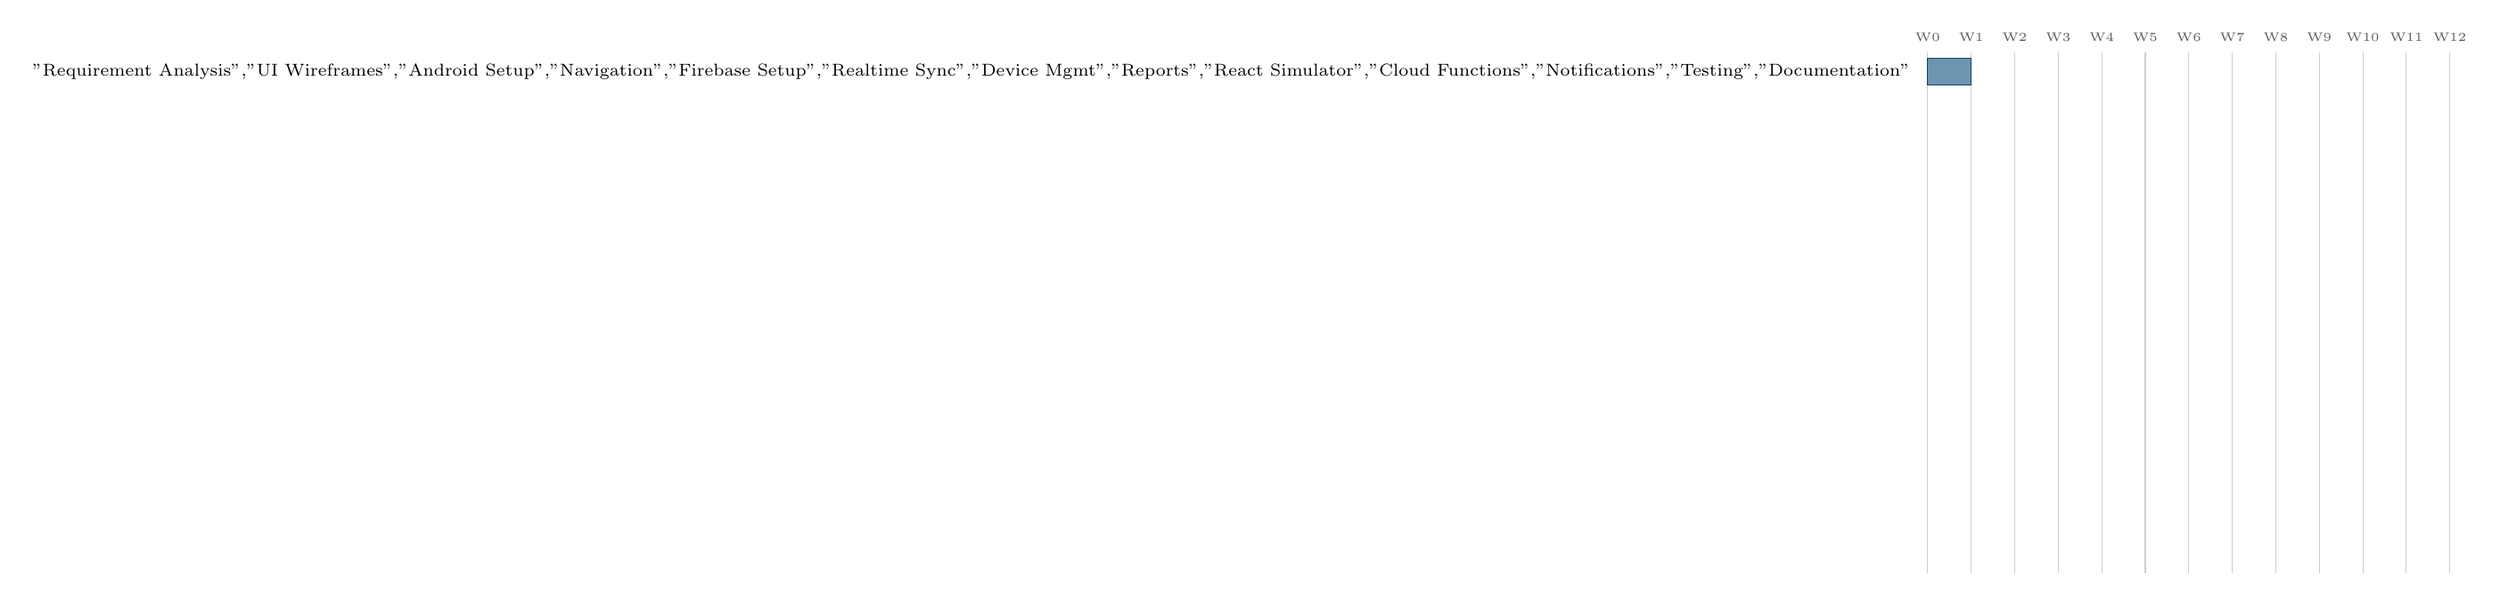
\begin{tikzpicture}[y=0.55cm, x=0.62cm]
\def\phases{{"Requirement Analysis","UI Wireframes","Android Setup","Navigation","Firebase Setup","Realtime Sync","Device Mgmt","Reports","React Simulator","Cloud Functions","Notifications","Testing","Documentation"}}
\def\starts{{0,1,1,2,2,3,4,6,5,7,8,9,10}}
\def\durs{{1,2,1,1,2,2,3,2,3,2,2,2,3}}

\foreach \w in {0,...,12} {
  \draw[lumagray!30] (\w,0) -- (\w,-13.5);
  \node[font=\tiny, text=lumagray] at (\w,0.4) {W\w};
}
\foreach [count=\i from 0] \p in \phases {
  \pgfmathsetmacro{\s}{ {\starts}[\i] }
  \pgfmathsetmacro{\d}{ {\durs}[\i] }
  \node[anchor=east, font=\scriptsize] at (-0.2,-\i-0.5) {\p};
  \filldraw[fill=lumaprimary!70, draw=lumasecondary] (\s,-\i-0.85) rectangle ({\s+\d},-\i-0.15);
}
\end{tikzpicture}
\caption{Gantt-style project timeline across a 12-week mini-project schedule.}
\label{fig:gantt}
\end{figure}

\subsection{Recommended Development Order}
Table~\ref{tab:dev-order} presents the recommended step-by-step development order used by the team, together with the milestone and expected output of each step.

\begin{longtable}{@{}p{0.6cm}p{3.0cm}p{4.6cm}p{4.6cm}@{}}
\toprule
\textbf{\#} & \textbf{Step} & \textbf{Milestone} & \textbf{Expected Output} \\
\midrule
\endhead
1 & Android project creation & Project builds and runs an empty Activity & A configured Android Studio project with Compose and Gradle set up \\
2 & UI development & Static screens render with placeholder data & Compose screens for all ten identified destinations \\
3 & Navigation & User can move between all static screens & A working \texttt{NavHost} with all routes registered \\
4 & Data models & Domain classes compile and are serializable & \texttt{Device}, \texttt{Floor}, \texttt{Room}, \texttt{Alert}, \texttt{Report} data classes \\
5 & Dashboard & Floor list renders from hard-coded data & Dashboard screen with add/edit/delete floor dialogs \\
6 & Floor management & Rooms and floor plan render correctly & Floor Details and Floor Plan screens \\
7 & Device management & All five device types have working controls & Device Details and Add Device screens \\
8 & Firebase integration & App reads/writes to a live Firebase project & Firebase project configured with initial Security Rules \\
9 & Realtime synchronization & Two clients see the same state change live & Repository classes with Realtime Database listeners \\
10 & React simulator & Simulator toggles devices and Android reflects it & Standalone React app with Device Cards and Status Chips \\
11 & Cloud Functions & Iron auto-shuts-off correctly in testing & Deployed Cloud Functions for automation \\
12 & Reports & Charts display aggregated usage data & Reports screen with bar/pie charts \\
13 & Notifications & Push notifications arrive on safety events & FCM integration and Notifications screen \\
14 & Testing & All test cases in Section~\ref{sec:testing} pass & Completed test execution log \\
15 & Documentation & Report and code comments finalized & This report and inline code documentation \\
\bottomrule
\caption{Recommended development order with milestones and expected outputs.}
\label{tab:dev-order}
\end{longtable}

% ============================================================
\section{Team Responsibilities}
\label{sec:team}

Luma was developed by a team of three members, with responsibilities divided along the natural boundaries between the Android application, the Firebase backend, and the React Hardware Simulator.

\begin{longtable}{@{}p{2.6cm}p{10.6cm}@{}}
\toprule
\textbf{Member} & \textbf{Primary Responsibilities} \\
\midrule
\endhead
Member 1 & Android UI (Jetpack Compose screens for all ten destinations), Navigation Compose graph, Dashboard implementation, Reports screen and charts. \\
Member 2 & Firebase project configuration, Realtime Database schema design and Security Rules, Realtime synchronization (Repository and listener implementation), Device Management screens and logic. \\
Member 3 & React Hardware Simulator Dashboard, Firebase Cloud Functions (automation logic), Testing (unit, integration, and synchronization test execution), Documentation (this report). \\
\bottomrule
\caption{High-level responsibility allocation across the three team members.}
\label{tab:team-responsibilities}
\end{longtable}

\subsection{Responsibility Matrix}
Table~\ref{tab:responsibility-matrix} cross-references each major project deliverable against the team member primarily responsible for it (P) and any member providing secondary support (S).

\begin{longtable}{@{}p{5.4cm}ccc@{}}
\toprule
\textbf{Deliverable} & \textbf{Member 1} & \textbf{Member 2} & \textbf{Member 3} \\
\midrule
\endhead
Android UI screens & P & S & -- \\
Navigation graph & P & -- & -- \\
Dashboard \& Floor Management & P & S & -- \\
Reports screen \& charts & P & -- & S \\
Firebase schema \& Security Rules & S & P & -- \\
Realtime synchronization (Repository/listeners) & S & P & S \\
Device Management (Add/Edit/Delete) & S & P & -- \\
React Hardware Simulator & -- & S & P \\
Cloud Functions (automation) & -- & S & P \\
Notifications (FCM integration) & S & S & P \\
Testing (all categories) & S & S & P \\
Documentation (this report) & S & S & P \\
\bottomrule
\caption{Responsibility matrix: P = Primary owner, S = Secondary support.}
\label{tab:responsibility-matrix}
\end{longtable}

% ============================================================
\section{Testing}
\label{sec:testing}

A multi-layered testing strategy was used to validate Luma across the Android application, the Firebase backend, and the React Hardware Simulator.

\subsection{Testing Categories}
\begin{longtable}{@{}p{3.2cm}p{10.0cm}@{}}
\toprule
\textbf{Category} & \textbf{Description} \\
\midrule
\endhead
Unit Testing & Kotlin unit tests for ViewModels (using fake Repository implementations) and JavaScript unit tests for React hooks and utility functions. \\
UI Testing & Jetpack Compose UI tests (\texttt{createComposeRule}) verifying that toggles, dialogs, and navigation actions behave as expected on Android; React Testing Library assertions for the simulator's Device Cards. \\
Integration Testing & Tests that exercise a Repository against a real (or emulated) Firebase project to confirm that reads/writes and listener callbacks behave correctly end-to-end. \\
Realtime Synchronization Testing & Manual and scripted tests that change a device's state on one client and assert that the change is observed on the other client within an acceptable latency window. \\
Firebase Testing & Validation of Security Rules using the Firebase Emulator Suite's Rules Unit Testing library, confirming that unauthorized reads/writes are correctly rejected. \\
Cloud Function Testing & Unit tests for Cloud Function handlers using the Firebase Functions Test SDK, and manual verification of the iron auto-shutdown timing behaviour. \\
Dashboard Testing & Manual exploratory testing of the React Hardware Simulator across supported browsers, confirming device cards render and toggle correctly. \\
User Acceptance Testing & Structured walkthroughs of each functional requirement in Section~\ref{sec:functional} performed by team members acting as end users. \\
\bottomrule
\caption{Testing categories applied to the Luma project.}
\label{tab:testing-categories}
\end{longtable}

\subsection{Representative Test Cases}
\begin{longtable}{@{}p{0.8cm}p{5.0cm}p{3.6cm}p{3.0cm}@{}}
\toprule
\textbf{ID} & \textbf{Test Case} & \textbf{Expected Result} & \textbf{Category} \\
\midrule
\endhead
TC-01 & Toggle a Smart Light ON from the Android app & Light state changes to ON in Firebase and on the Simulator within 1s & Synchronization \\
TC-02 & Turn Electric Iron ON and wait beyond max duration & Iron is automatically turned OFF and a push notification is received & Cloud Function \\
TC-03 & Simulator marks a device as disconnected & Android Notifications screen shows a ``Device disconnected'' alert & Cloud Function \\
TC-04 & Add a new floor from the Dashboard & New floor node appears under \texttt{/floors} and is visible on both clients & Integration \\
TC-05 & Attempt to write to \texttt{/devices} without authentication (where enabled) & Write is rejected by Firebase Security Rules & Firebase Rules \\
TC-06 & Toggle two switches on a 3-switch Multi-Switch Panel independently & Only the toggled switches change state; the third remains unaffected & UI \\
TC-07 & View Reports screen after several ON/OFF cycles & Bar and pie charts reflect the aggregated running time correctly & UI / Reports \\
TC-08 & Request a camera snapshot & A mock image URL is returned and displayed within the Device Details screen & Simulator \\
\bottomrule
\caption{Representative test cases and expected results.}
\label{tab:test-cases}
\end{longtable}

% ============================================================
\section{Security}
\label{sec:security}

\subsection{Firebase Security Rules}
Access to the Realtime Database is governed entirely by declarative \textbf{Firebase Security Rules}, evaluated by Firebase's servers on every read and write, independent of any client-side validation. This is essential in a Firebase-only architecture, since there is no custom API layer to otherwise enforce access control.

\begin{lstlisting}[language=json,caption={Simplified Firebase Realtime Database Security Rules for Luma.},label={lst:security-rules}]
{
  "rules": {
    "floors": {
      ".read": "auth != null",
      ".write": "auth != null"
    },
    "devices": {
      "$deviceId": {
        ".read": "auth != null",
        ".write": "auth != null",
        ".validate": "newData.hasChildren(['type','state','status'])"
      }
    },
    "alerts": {
      ".read": "auth != null",
      ".write": "auth != null || root.child('serviceAccount').exists()"
    },
    "reports": {
      ".read": "auth != null",
      ".write": false
    }
  }
}
\end{lstlisting}

\noindent The \texttt{reports} node is deliberately marked read-only for all clients, since report entries are exclusively generated by the Report Aggregator Cloud Function (Section~\ref{sec:cloudfunctions}), which operates with elevated Admin SDK privileges that bypass Security Rules.

\subsection{Authentication}
Firebase Authentication is included as an optional layer. When enabled, a single shared household account (email/password or Google sign-in) is used, consistent with Luma's single-user scope in this mini project; Section~\ref{sec:future} discusses extending this to per-member accounts.

\subsection{Realtime Security Considerations}
\begin{itemize}
    \item Security Rules are validated using the Firebase Emulator Suite before deployment, as described in Section~\ref{sec:testing}, to catch overly permissive or overly restrictive rules before they reach production.
    \item \texttt{.validate} rules enforce that device writes contain the expected required fields, reducing the risk of malformed data reaching either client.
    \item Because the Hardware Simulator and the Android app share the same authenticated identity in this mini project, Security Rules do not need to distinguish between the two client types; a production system would extend this with per-device-type or per-role rules.
\end{itemize}

\subsection{Cloud Function Security}
Cloud Functions execute using the Firebase Admin SDK, which operates with full read/write privileges to the Realtime Database, bypassing Security Rules entirely. Because Cloud Functions are only triggered by database events or an internal scheduler (never by direct client HTTP requests in this project), there is no publicly callable endpoint for an attacker to target, which reduces the attack surface compared to a custom REST API.

\subsection{Database Rules Summary}
\begin{longtable}{@{}p{2.6cm}p{4.8cm}p{5.4cm}@{}}
\toprule
\textbf{Node} & \textbf{Read Access} & \textbf{Write Access} \\
\midrule
\endhead
\texttt{/floors} & Authenticated users & Authenticated users \\
\texttt{/devices} & Authenticated users & Authenticated users (validated schema) \\
\texttt{/alerts} & Authenticated users & Authenticated users or the Admin SDK (Cloud Functions) \\
\texttt{/reports} & Authenticated users & Admin SDK only (Cloud Functions) \\
\bottomrule
\caption{Summary of database access rules by node.}
\label{tab:security-summary}
\end{longtable}

% ============================================================
\section{Future Improvements}
\label{sec:future}

While Luma satisfies the objectives defined for this mini project, several enhancements were identified as valuable directions for future work beyond the current scope:

\begin{longtable}{@{}p{3.6cm}p{9.6cm}@{}}
\toprule
\textbf{Improvement} & \textbf{Description} \\
\midrule
\endhead
Voice Assistant Integration & Integrate with Google Assistant and Amazon Alexa to allow voice-based device control, using their respective smart home SDKs on top of the existing Firebase data model. \\
Real Hardware (ESP32 / MQTT) & Replace the React Hardware Simulator with genuine ESP32-based microcontrollers communicating over MQTT, bridged into the same Firebase Realtime Database structure, allowing the Android app to work unchanged. \\
Face Recognition & Extend the Camera device type with on-device or cloud-based face recognition for visitor identification and enhanced security alerts. \\
Energy Analytics & Build richer analytics on top of the existing \texttt{/reports} node, including historical trend analysis and cost estimation based on local electricity tariffs. \\
AI Energy Optimization & Apply machine learning to historical usage data to suggest or automatically apply energy-saving schedules. \\
Multiple Users & Extend Firebase Authentication to support multiple household members with individual accounts and role-based permissions (e.g. adult vs. guest access). \\
Smart Sensors & Add support for passive sensor device types (temperature, humidity, motion, door/window contact) alongside the existing controllable device types. \\
Remote Access & Formalize secure remote access patterns (already partially supported by Firebase's cloud-hosted nature) with additional safeguards such as two-factor authentication for control actions performed away from the home network. \\
Weather Integration & Incorporate a weather API to inform automation rules, such as adjusting lighting schedules based on sunrise/sunset times or local conditions. \\
\bottomrule
\caption{Identified future improvements beyond the current project scope.}
\label{tab:future-improvements}
\end{longtable}

% ============================================================
\section{Conclusion}
\label{sec:conclusion}

Luma demonstrates that a fully functional, realtime, multi-client smart home platform can be built using a purely serverless, Firebase-centric architecture, without the need for a custom REST API, a dedicated application server, or physical IoT hardware. By separating the concerns of presentation (the Android application and the React Hardware Simulator), synchronization (the Firebase Realtime Database and its client SDKs), and automation (Firebase Cloud Functions and Cloud Messaging), the project achieves a clean, modular architecture that satisfies every objective defined in Section~\ref{sec:objectives}: live monitoring, responsive control, multi-floor and multi-device management, realtime synchronization across independent clients, safety automation for the Electric Iron, usage reporting, and a realistic substitute for physical hardware through the Hardware Simulator Dashboard.

The MVVM architecture adopted on the Android side, combined with the Repository pattern's encapsulation of Firebase-specific logic, produced a codebase that is testable, maintainable, and consistent with current Android development best practices. On the backend, Firebase Cloud Functions proved sufficient to implement all required automation -- most notably the safety-critical iron auto-shutdown feature -- entirely through database-triggered and scheduled execution, validating the architectural decision documented in Section~\ref{sec:architecture} to avoid a custom backend server.

Beyond meeting the immediate requirements of the SCS 3311 mini project, Luma's architecture is directly extensible toward a production-grade smart home system: the React Hardware Simulator could be replaced by genuine ESP32/MQTT-based hardware without any change to the Android application or the Firebase data model, and the features outlined in Section~\ref{sec:future} -- multi-user support, voice assistants, and AI-driven energy optimization -- can each be layered onto the existing foundation incrementally. The project therefore serves both as a complete academic deliverable and as a credible foundation for continued development.


\end{document}
